\documentclass[12pt]{ucthesis}

\usepackage{etex}
\usepackage[morefloats=125]{morefloats}
\usepackage[hyphens]{url}
\usepackage{subfig}
\usepackage{graphicx}
\usepackage{amssymb}
\usepackage{amsmath}
\usepackage[letterpaper]{geometry}
\usepackage[overload]{textcase}
\usepackage{color}
\usepackage[nonumberlist,toc]{glossaries}
\usepackage{wrapfig}
\usepackage{longtable}
\usepackage{morefloats}
\usepackage{float}
\usepackage{listings}
\usepackage{makecell}
\usepackage{appendix}
\usepackage[]{algorithm2e}
\usepackage{titlesec}
\usepackage[breaklinks=true,hidelinks,pdfusetitle]{hyperref}
\usepackage{cleveref}
\usepackage{ifthen}

\usepackage{siunitx}
\usepackage{pdfpages}
\usepackage{longtable}
\usepackage{pdflscape}
\usepackage{xcolor}
%\usepackage{setspace}

% Table related packages
\usepackage{tabularx}
\usepackage{booktabs}
\usepackage{ragged2e}  % for '\RaggedRight' macro (allows hyphenation)
\newcolumntype{Y}{>{\RaggedRight\arraybackslash}X} 

\makeindex
\makeglossaries

% Shrink the size of headers
\titleformat{\chapter}[display]
        {\normalfont\normalsize\centering}
        {\ifthenelse{\equal{\thechapter}{A}}{APPENDICES\\[4.3ex]}{}\chaptertitlename\ \thechapter}
        {0pt}{\normalsize\uppercase}
\titlespacing*{\chapter}{0pt}{-20pt}{4.3ex plus .2ex}


\titleformat*{\section}{\normalsize\bfseries}
\titleformat*{\subsection}{\small\bfseries}
\titleformat*{\subsubsection}{\small\bfseries}
\titleformat*{\paragraph}{\small\bfseries}
\titleformat*{\subparagraph}{\small\bfseries}

% Python formatting ~~~~~~~~~~~~~~~~~~~~~~~~~~~~~~~~~~~~~~~~~~~~~~~
% Default fixed font does not support bold face
\DeclareFixedFont{\ttb}{T1}{txtt}{bx}{n}{12} % for bold
\DeclareFixedFont{\ttm}{T1}{txtt}{m}{n}{12}  % for normal

% Custom colors
\usepackage{color}
\definecolor{deepblue}{rgb}{0,0,0.5}
\definecolor{deepred}{rgb}{0.6,0,0}
\definecolor{deepgreen}{rgb}{0,0.5,0}

\usepackage{linegoal,listings}

% Fixes inline wrapping issue, see https://tex.stackexchange.com/questions/56361/avoid-linebreak-in-lstinline-if-possible
\newsavebox{\mylisting}
\makeatletter
\newcommand{\lstInline}[2][,]{%
  \begingroup%
  \lstset{#1}% Set any keys locally
  \begin{lrbox}{\mylisting}\lstinline!#2!\end{lrbox}% Store listing in \mylisting
  \setlength{\@tempdima}{\linegoal}% Space left on line.
  \ifdim\wd\mylisting>\@tempdima\hfill\\\fi% Insert line break
  \lstinline!#2!% Reset listing
  \endgroup%
}
\makeatother

% C style
\newcommand\cstyle{\lstset{
	language=C,
	basicstyle=\ssp\ttfamily\tiny,
	frame=tb, % draw a frame at the top and bottom of the code block
 	tabsize=3, % tab space width
	showstringspaces=false, % don't mark spaces in strings
	numbers=left, % display line numbers on the left
	commentstyle=\color{deepgreen}, % comment color
	keywordstyle=\color{deepblue}, % keyword color
	stringstyle=\color{deepred}, % string color
	breaklines=true
}}

% C style for inline
\newcommand\cstyleinline{\lstset{
	language=C,
	basicstyle=\ssp\ttfamily,
	frame=tb, % draw a frame at the top and bottom of the code block
 	tabsize=3, % tab space width
	showstringspaces=false, % don't mark spaces in strings
	numbers=left, % display line numbers on the left
	commentstyle=\color{deepgreen}, % comment color
	keywordstyle=\color{deepblue}, % keyword color
	stringstyle=\color{deepred}, % string color
	breaklines=true
}}

% Command for inline C
\newcommand\cinline[1]{{\cstyleinline\lstInline{#1}}}

% C environment
\lstnewenvironment{clisting}[1][]
{
	\cstyle
	\lstset{#1}
}
{}

% Python style for highlighting
\newcommand\pythonstyle{\lstset{
		language=Python,
		basicstyle=\ttm,
		otherkeywords={self},             % Add keywords here
		keywordstyle=\ttb\color{deepblue},
		emph={MyClass,__init__},          % Custom highlighting
		emphstyle=\ttb\color{deepred},    % Custom highlighting style
		stringstyle=\color{deepgreen},
		frame=tb,                         % Any extra options here
		showstringspaces=false,            % 
		breaklines=true
}}

% Python environment
\lstnewenvironment{python}[1][]
{
	\pythonstyle
	\lstset{#1}
}
{}

% Python for external files
\newcommand\pythonexternal[2][]{{
		\pythonstyle
		\lstinputlisting[#1]{#2}}}

% Python for inline
\newcommand\pythoninline[1]{{\pythonstyle\lstinline!#1!}}



\bibliographystyle{abbrv}

\setlength{\parindent}{0.25in} \setlength{\parskip}{6pt}
\geometry{verbose,nohead,tmargin=1in,bmargin=1in,lmargin=1.5in,rmargin=1in}
\setcounter{tocdepth}{2}

% Different font in captions (single-spaced, bold) ------------
\newcommand{\captionfonts}{\small\bf\ssp}

\newcommand{\mycaption}[2]{\caption[#1 --- #2]{#1 --- #2}}

\makeatletter  % Allow the use of @ in command names
\long\def\@makecaption#1#2{%
  \vskip\abovecaptionskip
  \sbox\@tempboxa{{\captionfonts #1: #2}}%
  \ifdim \wd\@tempboxa >\hsize
    {\captionfonts #1: #2\par}
  \else
    \hbox to\hsize{\hfil\box\@tempboxa\hfil}%
  \fi
  \vskip\belowcaptionskip}
\makeatother   % Cancel the effect of \makeatletter
% ---------------------------------------

% Define Appendix refs
\crefname{app}{appendix}{appendices}
\Crefname{app}{Appendix}{Appendices}

\begin{document}

% Declarations for Front Matter
\title{Artificial Neural Network-Based Robotic Control}
\author{Justin Ng}
\degreemonth{June} \degreeyear{2018} \degree{Master of Science}
\defensemonth{June} \defenseyear{2018}
\numberofmembers{2}
   \chair{Andrew Danowitz, Ph.D. \linebreak Assistant Professor of Electrical Engineering}
   \othermemberA{Xiao-Hua Yu, Ph.D. \linebreak Professor of Electrical Engineering}
   \othermemberB{Fred W. DePiero, Ph.D. \linebreak Professor of Electrical Engineering}
\field{Electrical Engineering} \campus{San Luis Obispo}
\copyrightyears{seven}


\maketitle

\begin{frontmatter}

% Custom made for Cal Poly (by Mark Barry, modified by Andrew Tsui).
\copyrightpage

% Custom made for Cal Poly (by Andrew Tsui).
\committeemembershippage

\begin{abstract}
Artificial neural networks (ANNs) are highly-capable alternatives to traditional problem solving schemes due to their ability to solve non-linear systems with a non-algorithmic approach. The applications of ANNs range from process control to pattern recognition and, with increasing importance, robotics. This paper demonstrates continuous control of a robot using an actor-critic algorithm based on deep deterministic policy gradients (DDPG) originally conceived by Google DeepMind. The robot performs tasks such as locomotion within an enclosed area and object transportation. The paper also details the robot design process and explores the challenges of implementation in a real-time system.
\end{abstract}

\begin{acknowledgements}
\noindent
Thanks:
\begin{itemize}
    \item To Andrew Danowitz for his guidance, support, and time throughout the project. Many thanks!
    \item To my best friend in the world and unwavering fountain of support, Earth Wimolnit. You kept me alive and sane, and I couldn't have done it without you! Thank you and I love you!
\end{itemize}

\end{acknowledgements}

\tableofcontents

\listoftables

\listoffigures

% Add CHAPTER into table of contents.
\addtocontents{toc}{%
   \noindent CHAPTER
}

\end{frontmatter}

\pagestyle{plain}

\renewcommand{\baselinestretch}{1.66}

%\chapter{Introduction}

\textbf{Note}: All project files can be found at \url{https://www.github.com/okayjustin/roborodentia2017} \

\section{Definitions and Assumptions}
The robot is designed to only travel within a rectangular closed area of eight feet in the x direction and five feet in the y direction. The coordinate system is chosen as Cartesian with the origin placed at the bottom-left corner of the field. The position of the robot is always in the xy-plane since it cannot move vertically (z = 0). Therefore, $x$ refers to the robot position along the x-axis and ranges from 0 to 8 feet, and $y$ refers to position along the y-axis and ranges from 0 to 5 feet. Additionally, the robot can only rotate around the z-axis so $\theta$ refers to the angle of the robot in the xy-plane. Maintaining standard Cartesian coordinates, $\theta=\ang{0}$ is along the positive x direction while $\theta=\ang{90}$ is along the positive y direction.

\section{Cal Poly Roborodentia}
The robot is designed to compete in the 2018 Cal Poly Roborodentia, the university's annual intramural robotics competition, and thus conforms to its particular specifications and requirements. Briefly, autonomous robots collect and fire Nerf Rival Balls into nets to win points. A drawing of the field is shown below in Figure  \ref{fig:roborodentia_field}. 

\begin{figure}[H]   % [h] means here
	\centering
	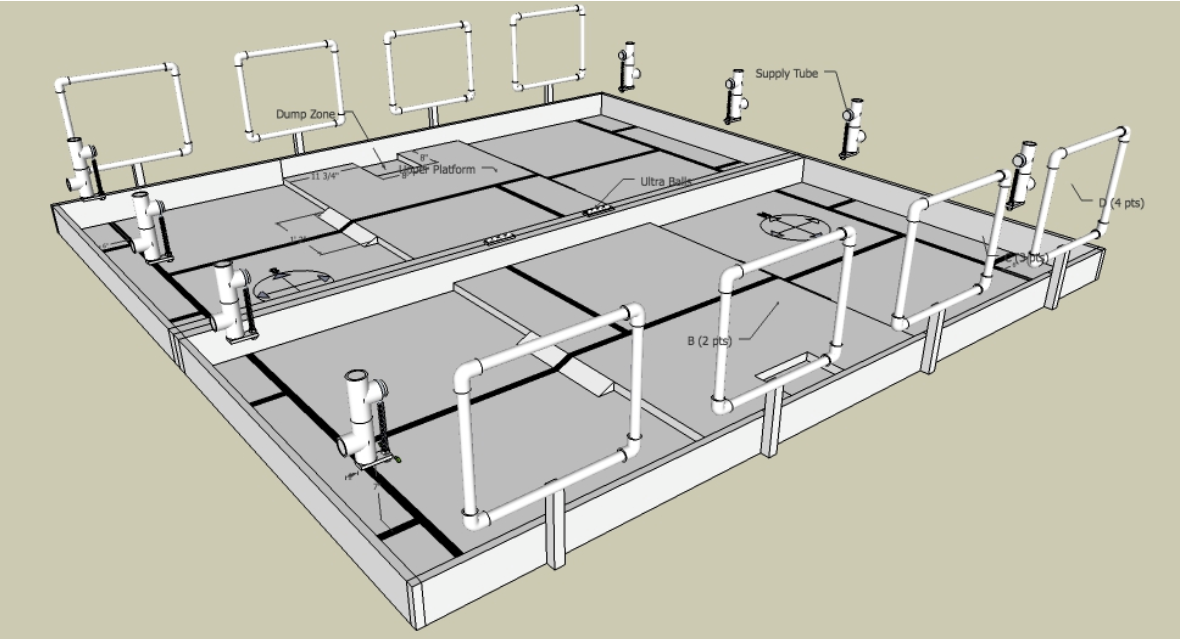
\includegraphics[width=7in]{figures/roborodentia_field.png}
	\caption{Roborodentia Field}
	\label{fig:roborodentia_field}
\end{figure}




\chapter{Mechanical Design}
%\chapter{Electrical Design}
\section{Introduction}



\section{Power}



\section{Sensors}



\section{Motor Drivers}


\section{Interconnect PCB}

\subsection{Schematic Capture}

\subsection{Board Layout}

\subsection{Assembly}

\subsection{Reworks}
%\chapter{Firmware Design}
\section{STM32CubeMX}
The robot uses an STMicroelectronics STM32F446RE microcontroller (MCU) for low level sensor interfacing and motor control signal generation. The MCU sends filtered sensor data to a Raspberry Pi \cite{raspberrypi} and receives speed and direction commands for each motor. Before starting the electrical design, the various hardware signals must be assigned to the MCU's GPIO with consideration for the device's peripherals such as timers and I\textsuperscript{2}C buses, a process aided by STMicroelectronics' configuration program, STM32CubeMX, shown in Figure \ref{fig:stm32cubemx} \cite{stm32cubemx}. Within the program, the user selects which MCU to configure and a graphical representation of the chip is shown in the GUI. The MCU's GPIO pins are arranged into banks of up to 16 pins each called ports. For example, PC2 is the second pin in Port C while PB11 is Pin 11 in Port B. The left column of the GUI lists the device peripherals including analog-to-digital converters (ADCs); various buses such as SPI, USART, and USB; and timers. Peripheral settings can be chosen here such as USART mode (asynchronous, single-wire, LIN, etc) and flow control as well as timer clock sourcing and channel modes.
\begin{figure}[H]   % [h] means here
	\centering 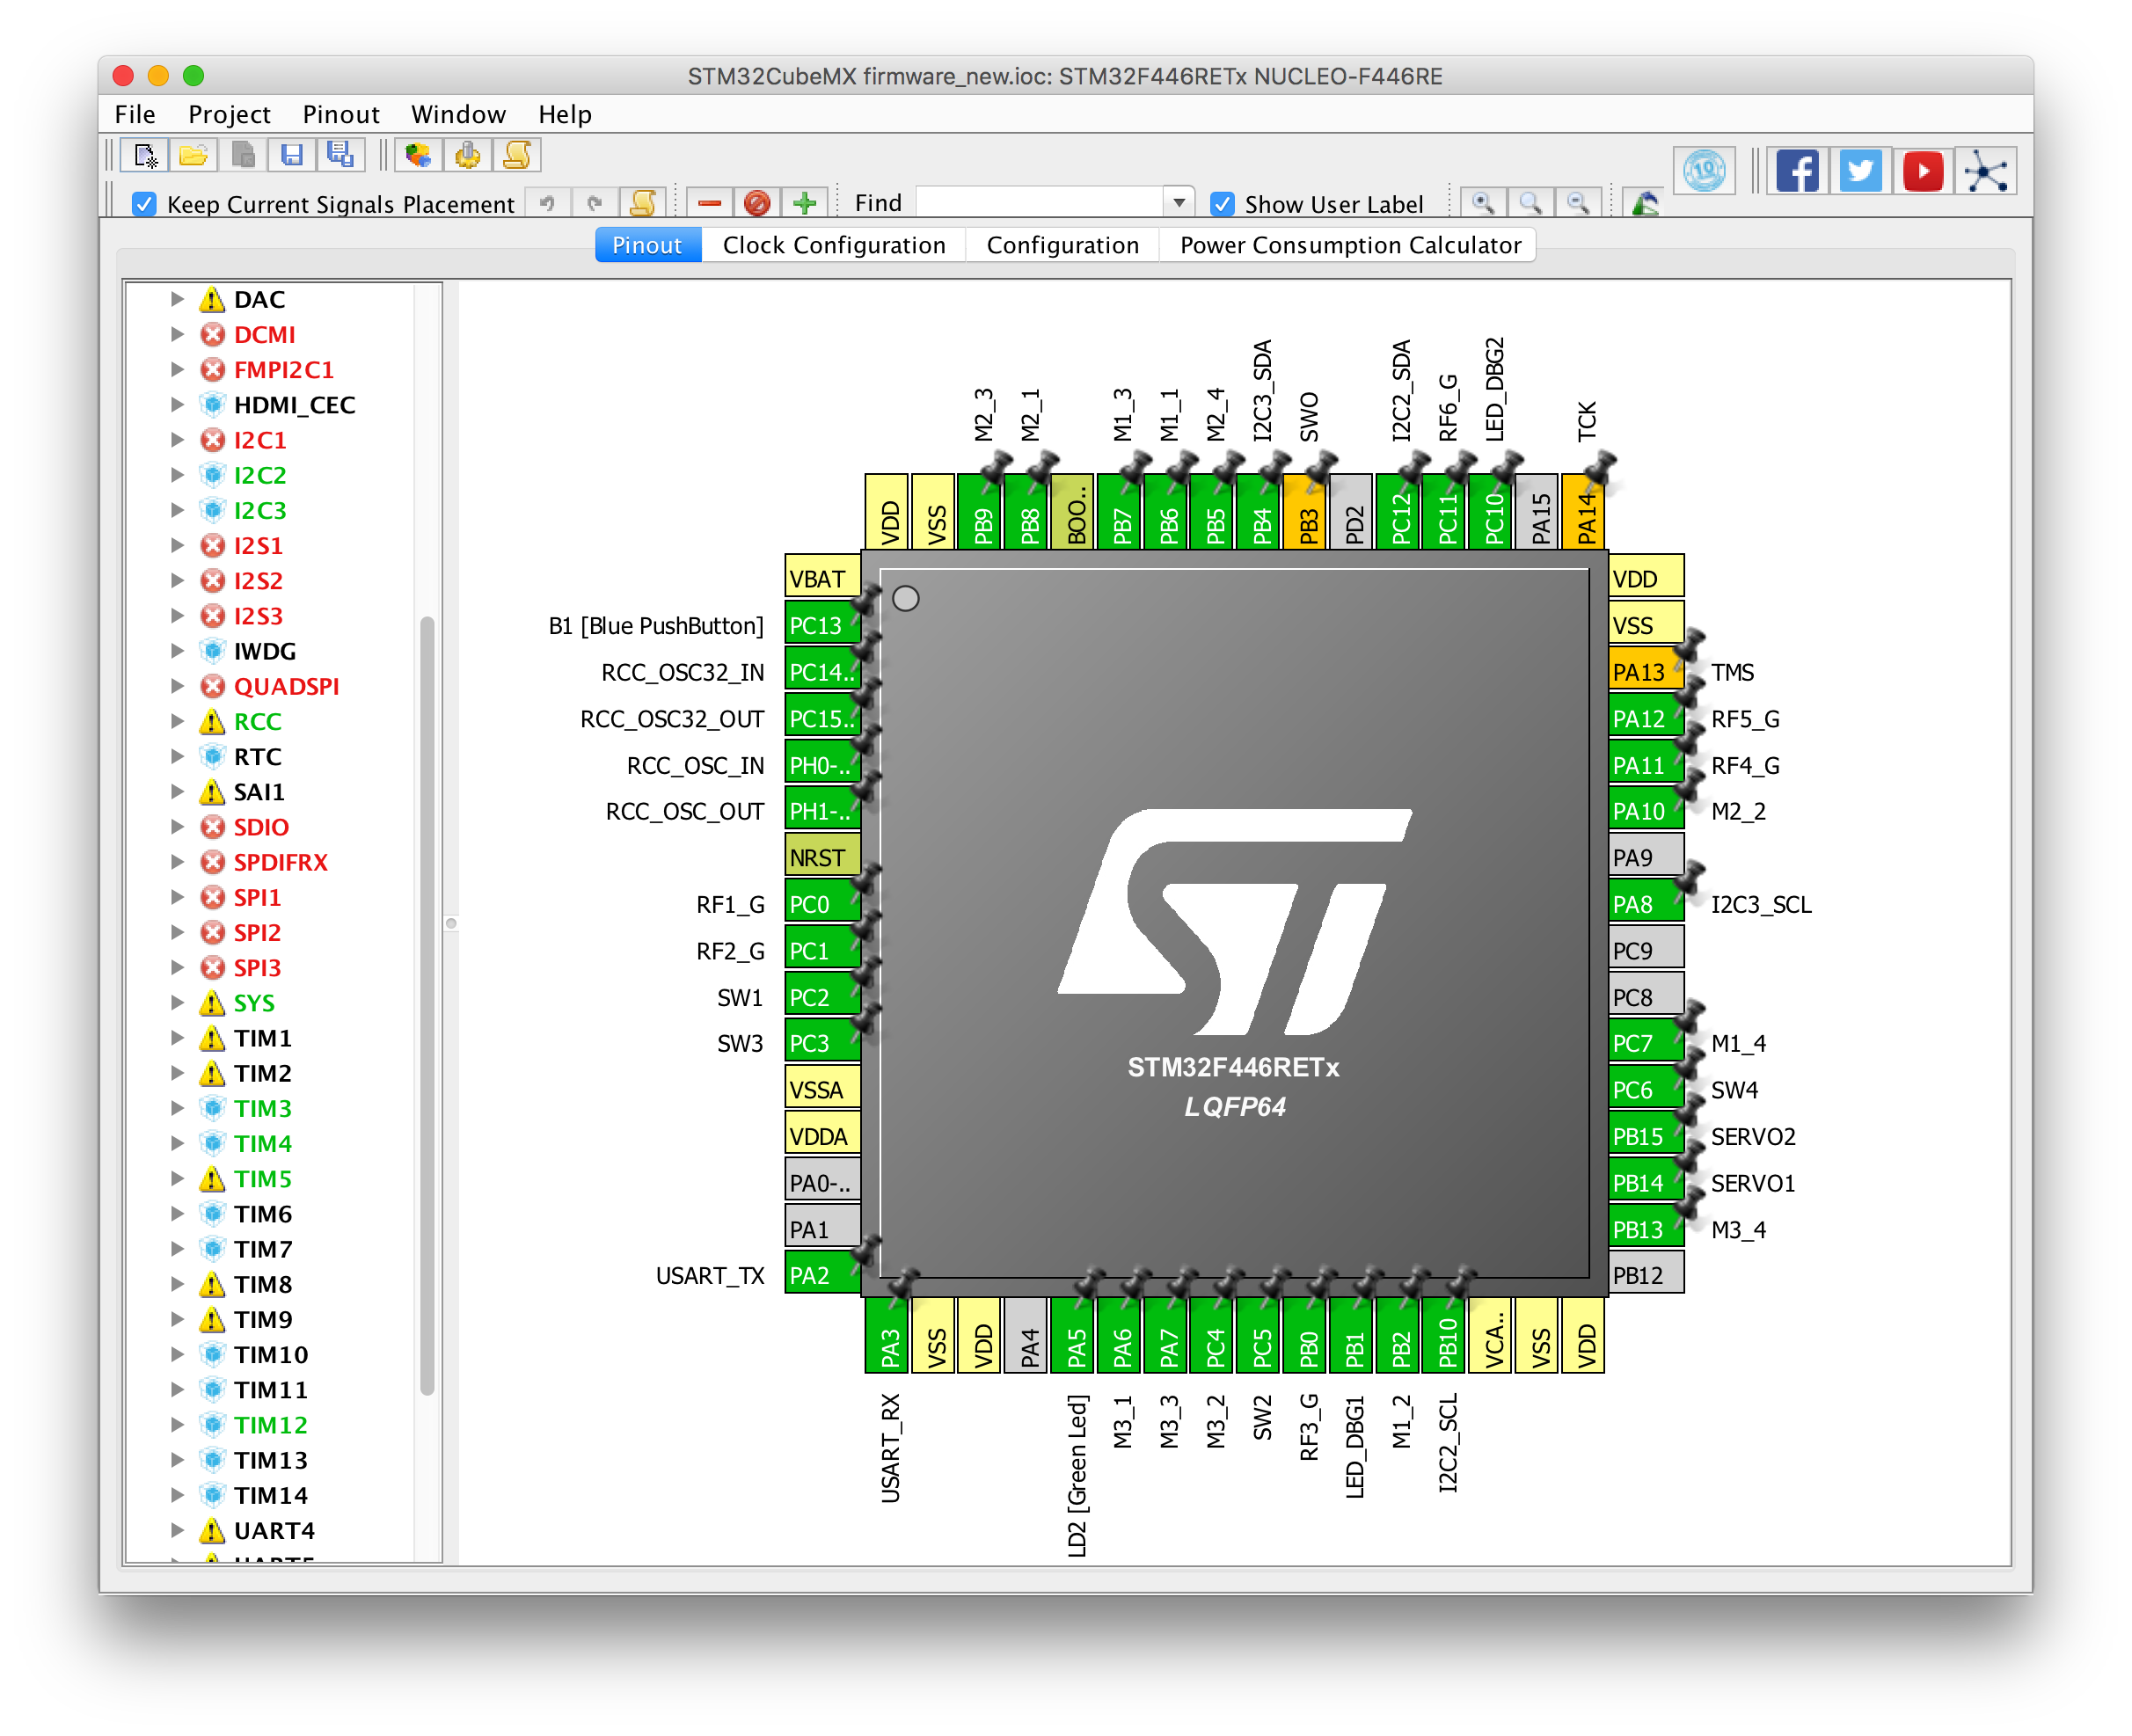
\includegraphics[width=6in, keepaspectratio]{figures/stm32cubemx.png}
	\caption{STM32CubeMX}\label{fig:stm32cubemx}
\end{figure}
The program greatly reduces development effort. Clicking a pin on the GUI brings up a menu of possible assignments. For example, clicking PB15, seen in Figure \ref{fig:stm32cubemx_pin}, shows that the pin can be used for the ADC, I2S2, as SPI2's MOSI, TIMER12's CH2 output, part of the USB differential data pair, as standard GPIO input or output, and more. As pins are assigned to various purposes, the program continually checks for compatibility issues and pin conflicts so a user can iteratively assign pins until all errors clear. For example, using a particular set of timers may actually prevent the use of I2C1 so either I2C2 or I2C3 must be used instead. This process is much faster and less error-prone than searching through the MCU's immense datasheet to manually check for assignment conflicts within every peripheral.
\begin{figure}[H]   % [h] means here
	\centering 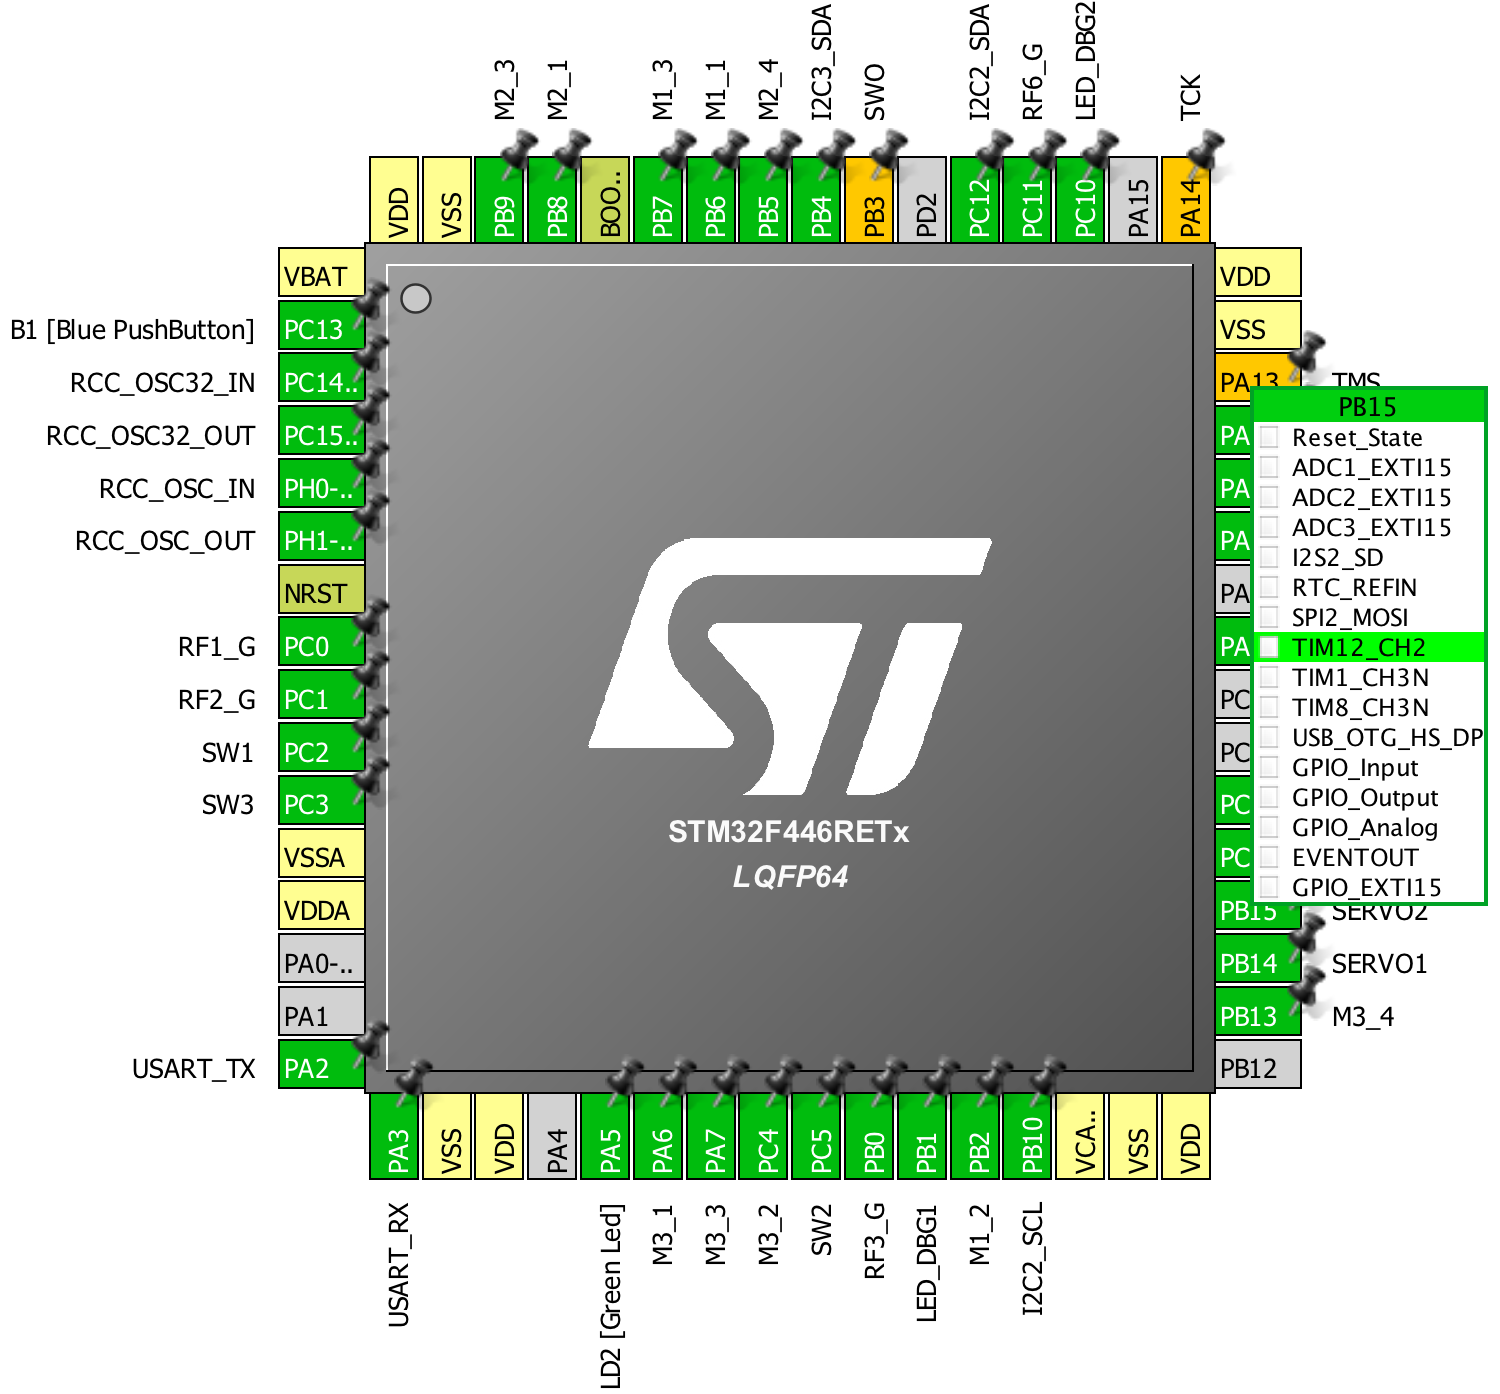
\includegraphics[width=6in, keepaspectratio]{figures/stm32cubemx_pin.png}
	\caption{STM32CubeMX -- Pin Menu}\label{fig:stm32cubemx_pin}
\end{figure}
The software also provides device-wide clock and PLL configuration as shown in Figure \ref{fig:stm32cubemx_clocks}. The MCU uses an external 8 MHz crystal to drive the internal PLL which then generates a 180 MHz system clock. Since the system is optimized for performance instead of power-saving, the advanced peripheral bus (APB) clocks run at 45 MHz and 90 MHz for APB1 and APB2, respectively \cite{stm32f446re}. 
\begin{figure}[H]   % [h] means here
	\centering 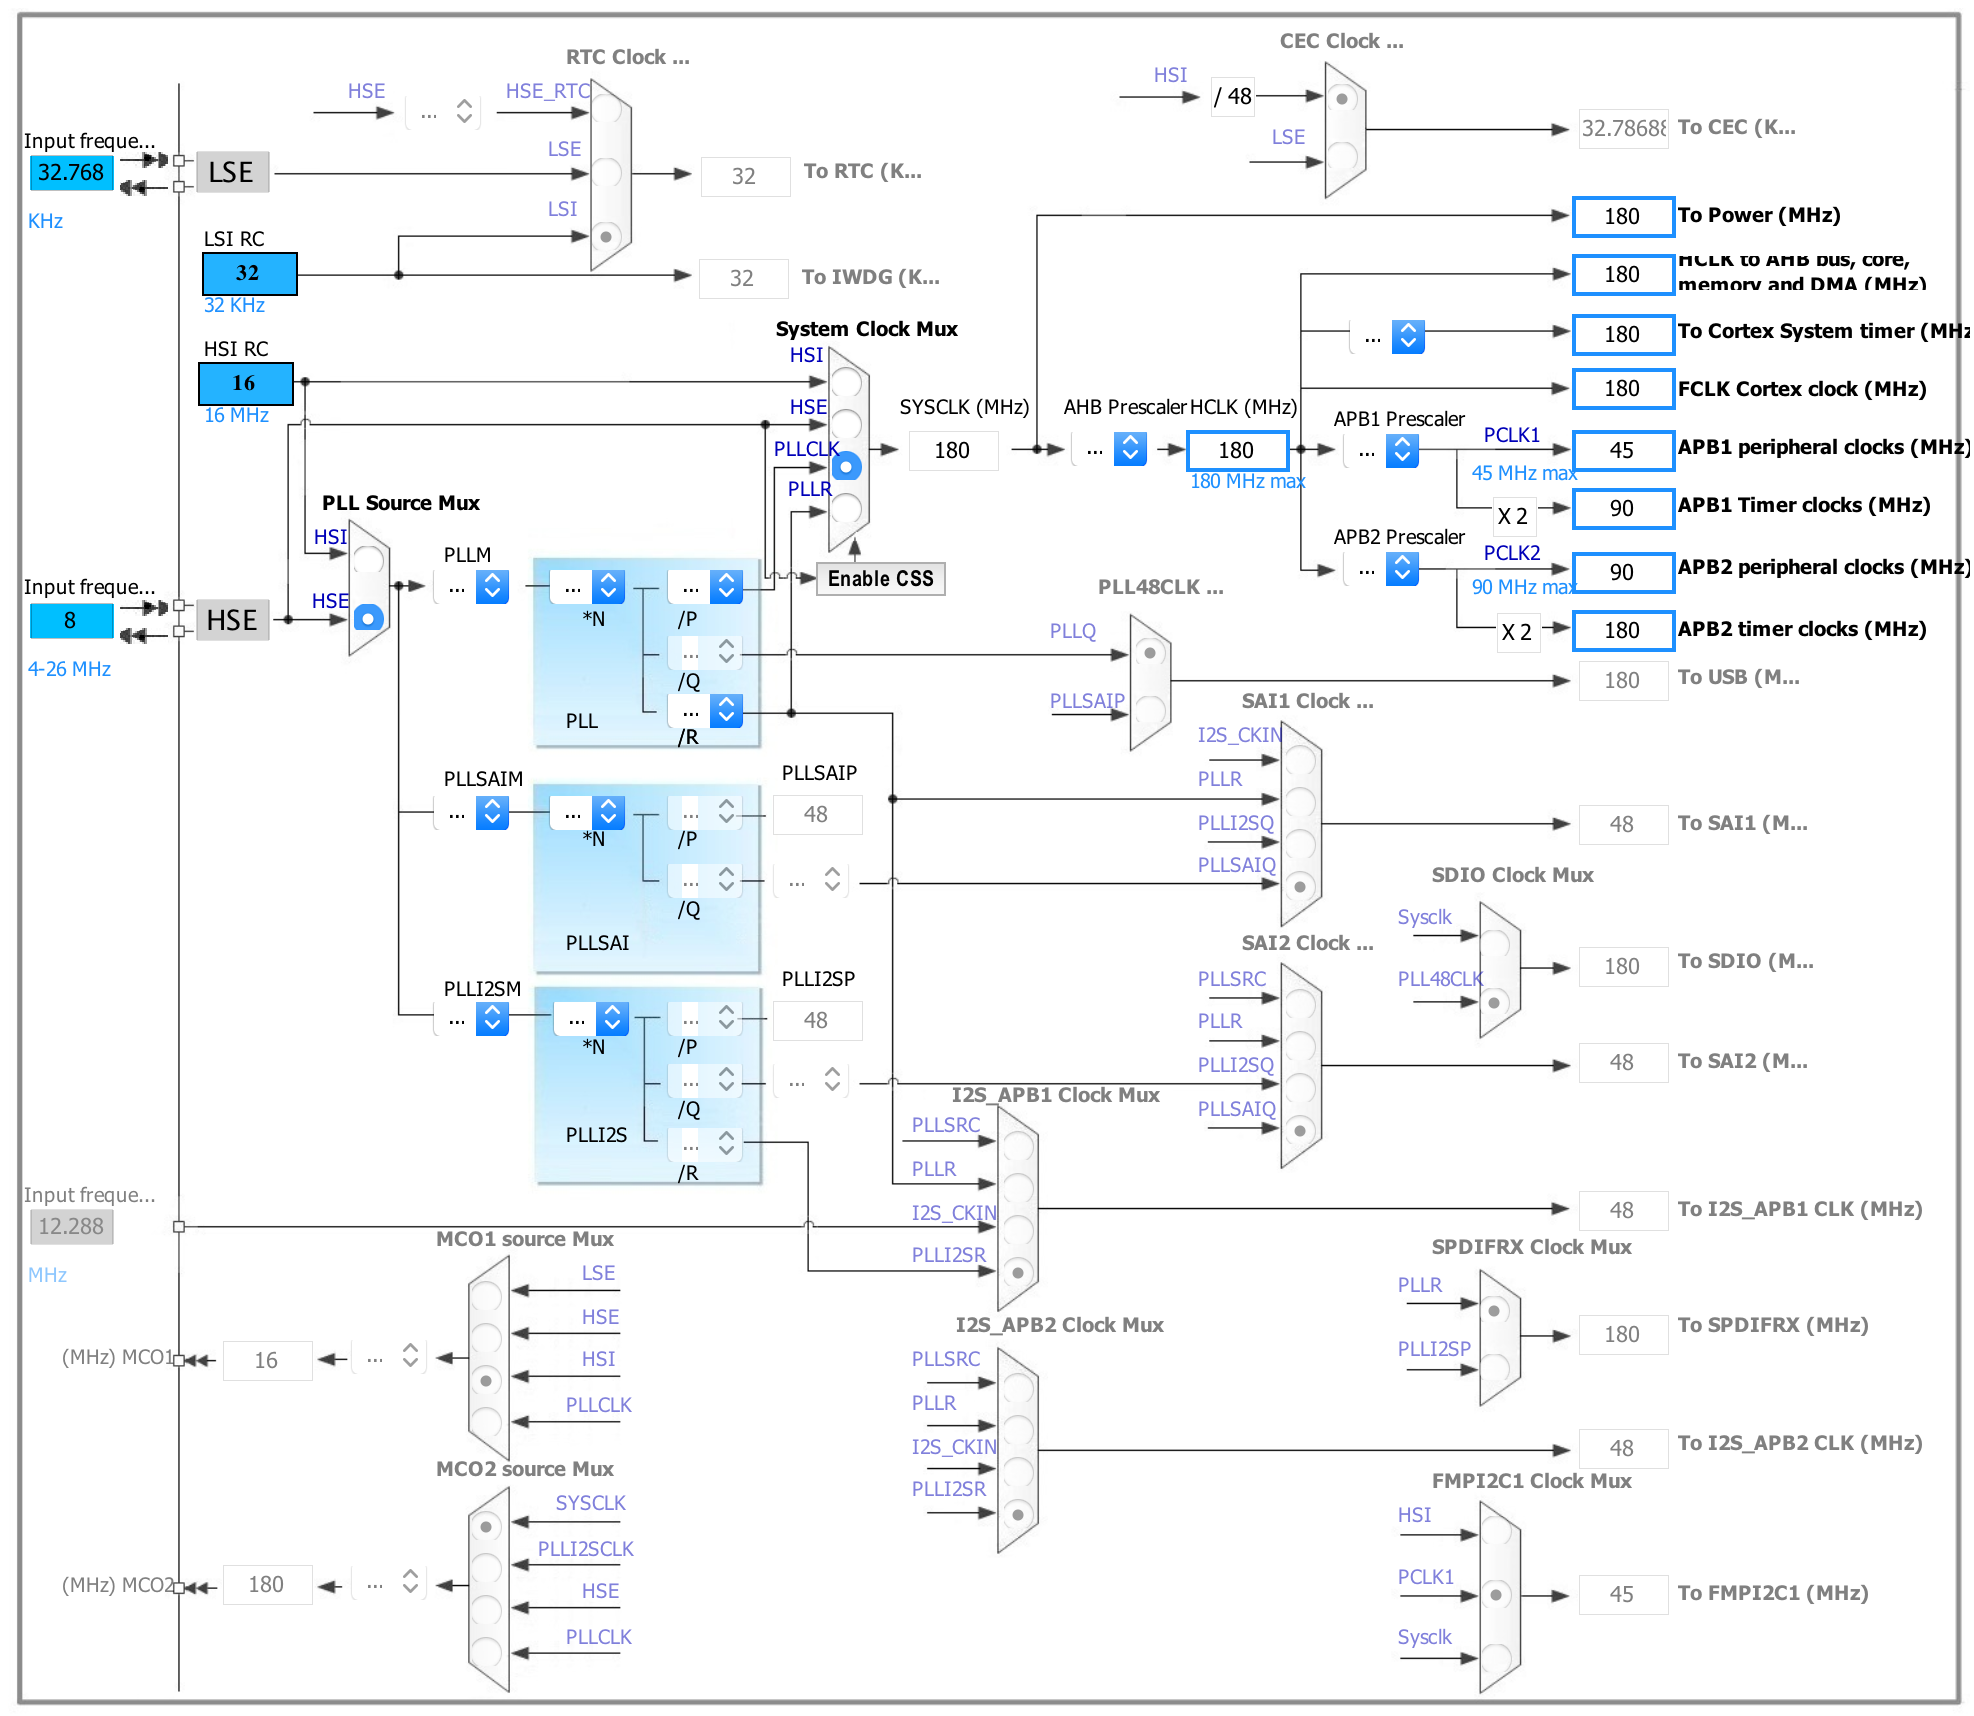
\includegraphics[width=6in, keepaspectratio]{figures/stm32cubemx_clocks.png}
	\caption{STM32CubeMX -- Clock Configurator}\label{fig:stm32cubemx_clocks}
\end{figure}
Another tab within STM32CubeMX provides detailed peripheral configuration, shown in Figure \ref{fig:stm32cubemx_config}. Both I\textsuperscript{2}C buses are set to 400 kHz with a 2:1 T\textsubscript{low}:T\textsubscript{high} duty cycle to meet the minimum pulse width requirement of slave devices. The USART peripheral is configured to 921,600 bits/s, 8-bit words, no parity, and one stop bit. The direct memory access (DMA) controller is set to process requests from the I\textsuperscript{2}C and UART peripherals to reduce processor load. 
\begin{figure}[H]   % [h] means here
	\centering 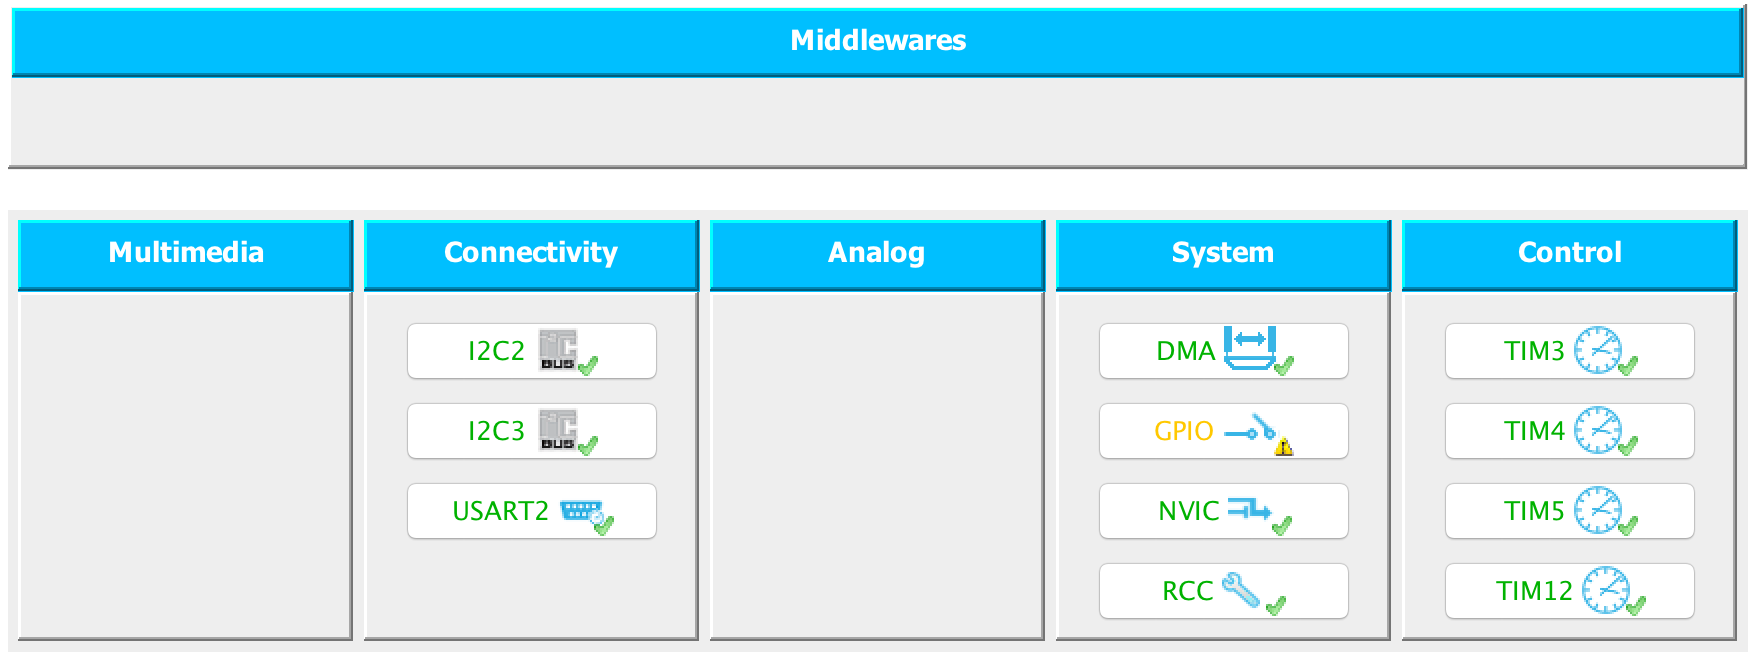
\includegraphics[width=6in, keepaspectratio]{figures/stm32cubemx_config.png}
	\caption{STM32CubeMX -- Peripheral Configurator}\label{fig:stm32cubemx_config}
\end{figure}
The robot uses four of the MCU's timers: TIMER3, TIMER4, TIMER5, and TIMER12. Each of these timers sources its base clock from the APB1 clock which is 90 MHz. TIMER3 and TIMER4 output 6 PWM control signals for the motor drivers. They are set to count upward and reset after the counter reaches 2047 to produce a 43.9 kHz PWM frequency in the ultrasonic range. TIMER5, used for delay and timing functions, employs a clock prescaler of 9000 so the counter increases every 0.1 ms and never resets; the 32-bit counter has a maximum value of 4,294,967,295 corresponding to a counter rollover period of about 5 days. Finally, TIMER12 drives the PWM signals for servo control. It uses a 45 prescaler and a 50,000 counter period to produce a 40 Hz PWM frequency.

After configuring the various items above, STM32CubeMX can generate common boilerplate plate code to initialize and configure all the devices. Include and source files are generated on a by-peripheral basis to compartmentalize code. The program also generates a report of the device configuration, attached in Appendix \ref{appendix:stm32cubemx_report}.

\section{Microcontroller Firmware}
The firmware, written in C and compiled with gcc, consists of a main file in conjunction with peripheral driver files \cite{gcc}. The dependency graph is shown in Figure \ref{fig:firmware_dependencies} with file descriptions shown in Table \ref{tab:firmware_file_desc}.  STM32CubeMX automatically generated several files to which user code was added for specific robot functions. The VL53L0X API, provided by STMicroelectronics, was also modified for the STM32F446 platform. Table \ref{tab:firmware_specs} lists the firmware requirements.
\begin{figure}[H]   % [h] means here
	\centering 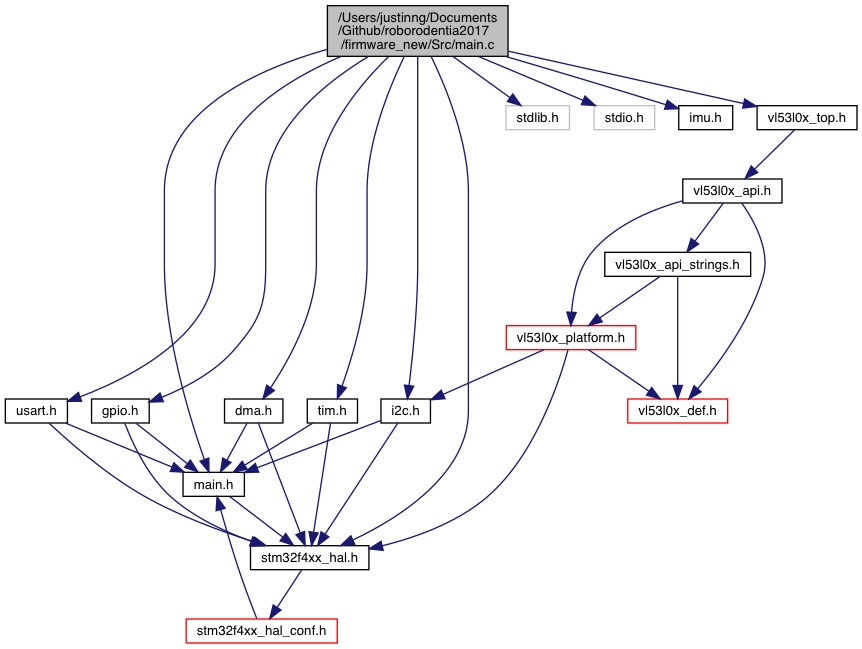
\includegraphics[width=6in,height=9in,keepaspectratio]{figures/firmware_dependencies.png}
	\caption{Firmware Dependency Graph for main.c}\label{fig:firmware_dependencies}
\end{figure}
\begin{table}[H]
	\centering	\caption{Firmware -- Source File Summary} 	\label{tab:firmware_file_desc}
	\begin{tabular}{r|l}
		\toprule 
		\multicolumn{1}{c}{File (.h/.c)} & \multicolumn{1}{c}{Description} \\ 
		\midrule 
		main & Initialization and main loop. \\  
		stm32f4xx\_hal & Hardware abstraction layer driver. \\  			
		dma & Sets up DMA priorities and enables DMA interrupts. \\  		
		i2c & Initializes I\textsuperscript{2}C buses, read/write, finds active devices. \\  		
		tim & Initializes timers 3, 4, 5, and 12. \\  		
		usart & Initializes UART, functions to write to bus, DMA callbacks. \\  		
		gpio & Configures GPIO modes (in/out), speeds, and pull-ups/pull-downs. \\  		
		vl53l0x\_top & STMicroelectronics API for configuring and reading rangefinders. \\  				 
		imu & Initializes IMU; read gyroscope, accelerometer, and magnetometer. \\ 
		\bottomrule 		
	\end{tabular} 
\end{table}
\begin{table}[H]
	\centering	\caption{Firmware -- Requirements} 	\label{tab:firmware_specs}
	\begin{tabular}{c|l}
		\toprule 
		 & \multicolumn{1}{c}{Requirements} \\ 
		 \midrule 
		1. & Initialize I\textsuperscript{2}C sensors including rangefinders and IMU. \\  
		2. & Read and store data from sensors. \\  
		3. & Filter data from sensors to reduce noise. \\  
		4. & Generate PWM signal to drive servo. \\  
		5. & Generate control signals to motor drivers. \\  
		6. & Sequence launcher motors, blower fan, and servo to fire balls. \\  
		7. & Flash LED to indicate error state. \\  
		8. & Communicate with computer over UART link. Add'l specifications in \ref{tab:firmware_uart_specs}. \\ \bottomrule 
	\end{tabular} 
\end{table}

\subsection{UART Commands}
The MCU responds to UART commands from a computer. The command syntax generally involves a sequence of one or more 8-bit characters. Table \ref{tab:firmware_uart_specs} lists the available commands. 
\begin{table}
	\centering	\caption{Firmware -- UART Commands}  \label{tab:firmware_uart_specs}
	\begin{tabularx}{\textwidth}{@{} c|Y @{}}
		\toprule 
		Syntax & \multicolumn{1}{c}{Command} \\ 
		\midrule 
		A & Start reading all rangefinders. \\  
		B & Returns sensor data in binary form (machine-readable). \\  
		D & Return sensor data in text form (human-readable). \\  
		I\textless BUS\textgreater & Scans I\textsuperscript{2}C bus and returns addresses of active devices. \\ 
		& \textless BUS\textgreater\ valid values: \\ 
		& \qquad 2 : Scan I2C2. \\
		& \qquad 3 : Scan I2C3. \\  \addlinespace
		L\textless SIDE\textgreater & Launch balls from one side of the hopper. \\
		& \textless SIDE\textgreater\ valid values: \\ 
		& \qquad L : Launch balls from left side. \\
		& \qquad R : Launch balls from right side. \\
		& \qquad S : Stop all motors. \\  \addlinespace
		M\textless FL\textgreater\textless BL\textgreater\textless BR\textgreater\textless FR\textgreater & Sets motor duty cycle calculated as \textless arg\textgreater\ divided by 2047. Each argument accepts a integer from 0 to 2047. \\
		& \textless FL\textgreater\ : PWM value for front left motor. \\
		& \textless BL\textgreater\ : PWM value for back left motor. \\
		& \textless BR\textgreater\ : PWM value for back right motor. \\
		& \textless FR\textgreater\ : PWM value for front right motor. \\  \addlinespace	
		V & Returns firmware version info. \\  
		Z & Return debug button pressed flag. \\ 
		\bottomrule 
	\end{tabularx} 
\end{table}

\subsubsection{UART Receiving}
After receiving a character on the UART bus, the DMA places it into \cinline{rxBuffer} and fires an interrupt. The MCU enters the UART receive complete DMA callback, shown in Listing \ref{list:uart_receive}, which collects the received characters into a command string stored in \cinline{stringBuffer}. If the UART receives a new line or line return character, the callback appends a null character to the string and calls \cinline{consoleCommand()} to parse and execute the command. The define \cinline{UART_RX_WRITEBACK} controls whether received characters and commands are echoed.
\begin{clisting}[caption={UART Receive Callback},label={list:uart_receive}]
#define RX_BUFFER_MAX_LENGTH 32 
#define UART_RX_WRITEBACK 0

uint8_t rxBuffer = '\000';
uint8_t stringBuffer[RX_BUFFER_MAX_LENGTH];
uint8_t stringBufferIndex;

void HAL_UART_RxCpltCallback(UART_HandleTypeDef *huart)
{
    uint8_t i;

    // Clear buffer
    if (stringBufferIndex == 0) {for (i = 0; i < RX_BUFFER_MAX_LENGTH; i++) stringBuffer[i] = 0;}	

    if ((rxBuffer != 10) && (rxBuffer != 13))	//if received data different from ascii 13 (enter)
    {
        if (stringBufferIndex < RX_BUFFER_MAX_LENGTH){
            stringBuffer[stringBufferIndex++] = rxBuffer; //add data to stringBuffer
        }
    }
    else // If received data = 10 or 13
    {
        if (stringBufferIndex < RX_BUFFER_MAX_LENGTH){
            stringBuffer[stringBufferIndex++] = '\0'; //add null char
        } else {
            stringBuffer[RX_BUFFER_MAX_LENGTH] = '\0'; //add null char
        }

        if (UART_RX_WRITEBACK){
            HAL_UART_Transmit(&huart2, (uint8_t *)&stringBuffer, stringBufferIndex, 0xFFFF);
            printf("\r\n");
        }
        consoleCommand((uint8_t *)&stringBuffer, stringBufferIndex);
        stringBufferIndex = 0;
    }

    if (UART_RX_WRITEBACK){
        HAL_UART_Transmit(&huart2, (uint8_t *)&rxBuffer, 1, 1);
    }
}
\end{clisting}

\subsubsection{UART Transmitting}
The \cinline{\_write()} function is overridden to redirect \cinline{printf()} output to UART using the code in Listing \ref{list:redirect_printf}.
\begin{clisting}[caption={Redirect printf()},label={list:redirect_printf}]
// Redirect printf to UART
int _write (int fd, char *ptr, int len) 
{ 
	transmitUART(ptr, len);
	return len; 
}
\end{clisting}

To avoid spending CPU cycles waiting for UART transmission to complete, the DMA buffers the character array directly to the peripheral. A flag, \cinline{txInProg}, prevents subsequent transmission until the UART transmit DMA callback, \cinline{HAL_UART_TxCpltCallback()}, clears the flag when the current transmission completes.
\begin{clisting}[caption={UART Transmit},label={list:uart_transmit}]
#define TX_BUFFER_MAX_LENGTH 2000 

uint8_t txBuffer[TX_BUFFER_MAX_LENGTH];
volatile uint8_t txInProg = 0;

// Transmit characters over UART
void transmitUART(char *ptr, int len)
{  
    // Check that the input isn't longer than our buffer
    if (len > TX_BUFFER_MAX_LENGTH){
        _Error_Handler(__FILE__, __LINE__);
    }
    // Wait until UART TX is finished
    while(txInProg == 1){}
    txInProg = 1;
    // Transfer the data to be sent into the txBuffer
    memcpy(txBuffer,(uint8_t *)ptr,len);
    HAL_UART_Transmit_DMA(&huart2, txBuffer, len); 
}

void HAL_UART_TxCpltCallback(UART_HandleTypeDef *huart)
{
    // Clear TX in progress flag when complete with transfer
    txInProg= 0;
}
\end{clisting}

\subsection{MCU Execution Flow}
The execution flow is as follows:
\begin{enumerate}
	\item Define and initialize a struct for motor pins and timer channels.
	\begin{clisting}[caption={Motor Struct},label={list:motor_struct}]
struct motor_t {
    GPIO_TypeDef *GPIOx;
    uint16_t GPIO_Pin;
    GPIO_PinState PinState;

    TIM_HandleTypeDef *TIM_Handle;
    TIM_OC_InitTypeDef sConfigOC;
    uint32_t TIM_Channel;
};

struct motor_t motorConfigs[4] = { 
    {MOTOR_FL_DIR_GPIO_Port, MOTOR_FL_DIR_Pin, GPIO_PIN_RESET, 0, {0}, TIM_CHANNEL_2}, 
    {MOTOR_FR_DIR_GPIO_Port, MOTOR_FR_DIR_Pin, GPIO_PIN_RESET, 0, {0}, TIM_CHANNEL_4}, 
    {MOTOR_BR_DIR_GPIO_Port, MOTOR_BR_DIR_Pin, GPIO_PIN_RESET, 0, {0}, TIM_CHANNEL_1}, 
    {MOTOR_BL_DIR_GPIO_Port, MOTOR_BL_DIR_Pin, GPIO_PIN_RESET, 0, {0}, TIM_CHANNEL_3}}; 
struct motor_t* motorConfigsPtr = motorConfigs;
	\end{clisting}
	\item Instantiate some variables.
	\begin{clisting}[caption={Communications Variables Initialization},label={list:comms_var_init}]
unsigned char data_packet[21];				// Holds sensor data for UART transmission
volatile uint8_t wd_reset = 0;				// Watchdog reset flag
volatile uint8_t sensor_update_req = 0;		// Queue rangefinder read flag
volatile uint8_t dbg_btn_latch = 0;			// Debug button latch
	\end{clisting}
	\item Enable all clocks since power saving not necessary.
	\begin{clisting}[caption={Enabling Clocks},label={list:enable_clocks}]
RCC->AHB1ENR |= 0xFFFFFFFF;
RCC->AHB2ENR |= 0xFFFFFFFF;
RCC->AHB3ENR |= 0xFFFFFFFF;
RCC->APB1ENR |= 0xFFFFFFFF;
RCC->APB2ENR |= 0xFFFFFFFF;
	\end{clisting}
	\item Reset peripherals, initialize SysTick, set up PLL and clocks.
	\begin{clisting}[caption={HAL and System Clock Initialization},label={list:hal_sysclk_init}]
HAL_Init();
SystemClock_Config();
	\end{clisting}
	\item Initialize configured peripherals.
	\begin{clisting}[caption={Peripheral Initialization},label={list:periph_init}]
MX_GPIO_Init();
MX_DMA_Init();
MX_I2C2_Init();
MX_I2C3_Init();
MX_TIM3_Init();
MX_TIM4_Init();
MX_TIM12_Init();
MX_USART2_UART_Init();
MX_TIM5_Init();
	\end{clisting}
	\item Reset system timer, enable UART receive DMA, initialize sensors.
	\begin{clisting}[caption={UART Service and Sensor Initialization},label={list:uart_sensor_init}]
TimeStamp_Reset();
serviceUART();
printf("Enabling IMU...\r\n");
IMU_begin();
printf("Initializing rangefinders...\r\n");
VL53L0X_begin();
	\end{clisting}
	\item Set servo to starting position.
	\begin{clisting}[caption={Servo Default Position},label={list:servo_default}]
if (HAL_TIM_PWM_Start(&htim12, TIM_CHANNEL_1) != HAL_OK){ Error_Handler(); }
	\end{clisting}
	\item Initialize variables and begin main loop.
	\begin{clisting}[caption={Loop Variables and Start},label={list:loop_start}]
uint32_t wd_start = 0;		// Watchdog start time
uint32_t cur_time = 0;		// Current time
uint8_t wd_en = 0;			// Watchdog enable
data_packet[20] = '\n';		// 21 byte sensor data packet to send over UART

while (1)
{
	\end{clisting}
	\item Watchdog prevents motors from running when UART is inactive. Receiving any UART command sets \cinline{wd\_reset} to 1.
	\begin{clisting}[caption={Motor Watchdog},label={list:motor_watchdog}]
	// Reset watchdog start time if flag is set
	if (wd_reset == 1){
		wd_start = TimeStamp_Get();  // Units of 0.1 ms based on Timer5
		wd_en = 1;
		wd_reset = 0;
	} else if (wd_en == 1){
		// Trigger if watchdog is enabled and expires
		cur_time = TimeStamp_Get();
		if ((cur_time - wd_start) > WD_LEN){
			wd_en = 0;
			
			// Disable motors
			int i;
			for (i=0; i<4; i++) {
				motorConfigs[i].PinState = GPIO_PIN_RESET;
				motorConfigs[i].sConfigOC.Pulse = 0; 
			}
			for (i=0; i<4; i++) {
				// Alter the PWM duty cycle and start PWM again
				if (HAL_TIM_PWM_ConfigChannel(motorConfigs[i].TIM_Handle, &motorConfigs[i].sConfigOC,
					motorConfigs[i].TIM_Channel) != HAL_OK) { Error_Handler(); }
				if (HAL_TIM_PWM_Start(motorConfigs[i].TIM_Handle, motorConfigs[i].TIM_Channel)
					!= HAL_OK){ Error_Handler(); }
				
				// Set the direction pin
				HAL_GPIO_WritePin(motorConfigs[i].GPIOx, motorConfigs[i].GPIO_Pin, motorConfigs[i].PinState);
			}
		}
	}											
	\end{clisting}
	\item Read debug tactile button state and latch it until read by UART.
	\begin{clisting}[caption={Debug Button Latch},label={list:dbg_btn_latch}]
	// Read debug button
	dbg_btn_latch = HAL_GPIO_ReadPin(B1_GPIO_Port, B1_Pin) && dbg_btn_latch;
	\end{clisting}
	\item If requested over UART, read all four rangefinders and store the data in the \cinline{data\_packet}.
	\begin{clisting}[caption={Rangefinder Read},label={list:range_read}]
	if (sensor_update_req == 1){
		int i;
		for (i = 0; i < 4; i++){
			if (rangefinderRead(i)){
				data_packet[i*2  ] = (rangeData[i] >> 8) & 0xFF;
				data_packet[i*2+1] =  rangeData[i]       & 0xFF;
			}
		}
		sensor_update_req = 0;
	}	
	\end{clisting}
	\item Read the magnetometer and store the data in the data packet.
	\begin{clisting}[caption={Magnetometer Read},label={list:mag_read}]
	magnetometer_read();
	data_packet[ 8] = (magData.x >> 8) & 0xFF;
	data_packet[ 9] =  magData.x       & 0xFF;
	data_packet[10] = (magData.y >> 8) & 0xFF;
	data_packet[11] =  magData.y       & 0xFF;
	data_packet[12] = (magData.z >> 8) & 0xFF;
	data_packet[13] =  magData.z       & 0xFF;	
	\end{clisting}
	\item Read the accelerometer and store the data in the data packet.
	\begin{clisting}[caption={Accelerometer Read},label={list:acc_read}]
	accelerometer_read();
	data_packet[14] = (accelData.x >> 8) & 0xFF;
	data_packet[15] =  accelData.x       & 0xFF;
	data_packet[16] = (accelData.y >> 8) & 0xFF;
	data_packet[17] =  accelData.y       & 0xFF;
	data_packet[18] = (accelData.z >> 8) & 0xFF;
	data_packet[19] =  accelData.z       & 0xFF;
}	
	\end{clisting}		
	\item Return to start of loop.
\end{enumerate}

\subsection{Error Handler}
During errors or faults, the MCU enters the error handler, prints an error message, and flashes the debug LED at 5 Hz.
\begin{clisting}[caption={Error Handler},label={list:error_handler}]
void _Error_Handler(char * file, int line)
{
	printf("Entered error handler.\r\n");
	while(1) 
	{
		HAL_GPIO_TogglePin(GPIOB, GPIO_PIN_1);
		HAL_Delay(100);
	}
}
\end{clisting}

%\chapter{Software Design}
All of the software running on the off-robot computer is written in Python in order to take advantage of the ease of development, library selection, and primarily the availability of TensorFlow, an open source machine learning framework.

\section{Definitions and Assumptions}
The robot is designed to only travel within a rectangular closed area of eight feet in the x direction and five feet in the y direction. The coordinate system is chosen as Cartesian with the origin placed at the bottom-left corner of the field. The position of the robot is always in the xy-plane since it cannot move vertically (z = 0). Therefore, $x$ refers to the robot position along the x-axis and ranges from 0 to 8 feet, and $y$ refers to position along the y-axis and ranges from 0 to 5 feet. Additionally, the robot can only rotate around the z-axis so $\theta$ refers to the angle of the robot in the xy-plane. Maintaining standard Cartesian coordinates, $\theta=\ang{0}$ is along the positive x direction while $\theta=\ang{90}$ is along the positive y direction.

\section{Kalman Filters}
The system relies on several different sensors to determine where it is within the environment, a problem commonly referred to as robot localization. The \textit{Kalman Filter} (KF), an optimal state estimator, performs noise filtering and sensor fusion, the process of combining measurements from multiple sensors. The filter operates on the principles of Bayesian inference and uses statistically noisy measurements over time and knowledge of the system to produce a more accurate estimate of an unknown variable than with measurement alone.

\subsection{Algorithm}
The Kalman Filter algorithm and equations are reproduced here from Roger Labbe's excellent interactive online book \cite{labbe_2017}.  The algorithm consists of two stages (not including initialization): prediction and update. During the first stage, the filter uses the current state and a process model (typically a function of time) to estimate the state in the next time step along with its uncertainty. The second stage uses sensor measurements to update the estimation by taking a weighted average based on the ratio of uncertainty between the prediction and measurement. 

\subsubsection*{Initialization}
Before the first run of the filter, initialize the estimated state (\textbf{x}, also called the posterior) and estimated state covariance matrix (\textbf{P}).
\subsubsection*{Predict}
During the predict phase, the process model is used to predict the future state (known as the prior) (\textbf{\=x}) after one time step by summing the posterior (\textbf{x}) multiplied by the \textit{state transition function} (\textbf{F}) with the control input model (\textbf{B}) multiplied by the control input (\textbf{u}). The covariance of prior (\textbf{\=P}) is larger than the posterior covariance (\textbf{P}) due to uncertainty in the process model (\textbf{Q}).
\begin{align*}
\bar{\textbf{x}} &= \textbf{Fx} + \textbf{Bu}\\
\bar{\textbf{P}} &= \textbf{FPF}^T + \textbf{Q}\\
\end{align*}

\subsubsection*{Update}
Make measurements (\textbf{z}, measurement mean) and determine their accuracy (\textbf{R}, measurement noise covariance). Calculate the residual (or difference) (\textbf{y}) between the measurement and the product of the measurement function (\textbf{H}) and the prior from the previous phase. \textbf{H} converts the prior from the state space to the measurement space. Calculate the weighting factor (\textbf{K}, Kalman gain), valued between 0 and 1, based on the whether the measurement or prior is more accurate. Set the new posterior, \textbf{x}, to an average of the measurement and prior, weighted by \textbf{K}. Finally, update the posterior's covariance, \textbf{P}, based on the measurement certainty. The algorithm then loops back to the predict phase using the newly-calculated posterior.
\begin{align*}
\textbf{y} &= \textbf{z} - \textbf{H}\bar{\textbf{x}}\\
\textbf{K} &= \bar{\textbf{P}}\textbf{H}^T(\textbf{H}\bar{\textbf{P}}\textbf{H}^T+\textbf{R})^{-1}\\
\textbf{x} &= \bar{\textbf{x}} + \textbf{Ky}\\
\textbf{P} &= (\textbf{I}-\textbf{KH})\bar{\textbf{P}}\\
\end{align*}

\subsection{Design}
The desired state variable \textbf{x} is chosen as the linear position, velocity, and acceleration in the x and y directions as well as the angular position, velocity, and acceleration about the z-axis:
\begin{align*}
\textbf{x} &= [x\ y\ \theta]^T\\
\dot{\textbf{x}} &= [\dot{x}\ \dot{y}\ \dot{\theta}]^T\\
\ddot{\textbf{x}} &= [\ddot{x}\ \ddot{y}\ \ddot{\theta}]^T\\
\end{align*}
The process model for position and velocity:
\[ \begin{cases} 
\bar{x}=x+\dot{x}\Delta t+0.5\ddot{x}(\Delta t)^2\\
\bar{\dot{x}}=\dot{x}+\ddot{x}\Delta t\\
\bar{\ddot{x}}=\ddot{x}\\
\end{cases} \]
Which can be written in the form:
\begin{align*}
\begin{bmatrix}\bar{x}\\ \bar{\dot{x}}\\ \bar{\ddot{x}} \end{bmatrix} &=
\begin{bmatrix}1 & \Delta t & 0.5(\Delta t)^2 \\
0 & 1 & \Delta t \\
0 & 0 & 1 \\\end{bmatrix}
\begin{bmatrix}x\\ \dot{x}\\ \ddot{x} \end{bmatrix}\\ 
\bar{\textbf{x}}&=\textbf{F}\textbf{x}
\end{align*}
The measurement vector is chosen as:
\[\textbf{z}=
\begin{bmatrix}z_x & z_{\ddot{x}} & z_y & z_{\ddot{y}} & z_{\theta} & z_{\dot{\theta}} \end{bmatrix}^T\]
The measurement noise matrix is shown below. The off-diagonals are 0 because the noise between sensors is assumed to be uncorrelated.
\[\textbf{R}=
\begin{bmatrix}\sigma^2_x & 0 & 0 & 0 &0 & 0\\
0 & \sigma^2_{\ddot{x}} & 0 & 0 & 0 & 0\\
0 & 0 & \sigma^2_y & 0 & 0 & 0 \\
0 & 0 & 0 & \sigma^2_{\ddot{y}} & 0 & 0\\
0 & 0 & 0 & 0 & \sigma^2_{\theta} & 0\\
0 & 0 & 0 & 0 & 0 & \sigma^2_{\dot{\theta}} \end{bmatrix}\]
%\chapter{Neural Network Design}
%\chapter{Conclusion}

Placeholder.


\nocite{*}
\bibliography{bibliography}

% Indents Appendix in Table of Contents
\makeatletter
\addtocontents{toc}{\let\protect\l@chapter\protect\l@section}
\makeatother

% Hack to make Appendices to appear in Table of Contents
\addtocontents{toc}{%
   \noindent APPENDICES
}
\begin{appendices}
\chapter{Mechanical Parts -- Bill of Materials}
\label{appendix:mech_bom}

\LTXtable{\textwidth}{tables/tab_mech_bom.tex}


\chapter{Interconnect PCB Schematic}
\label{appendix:schematic}
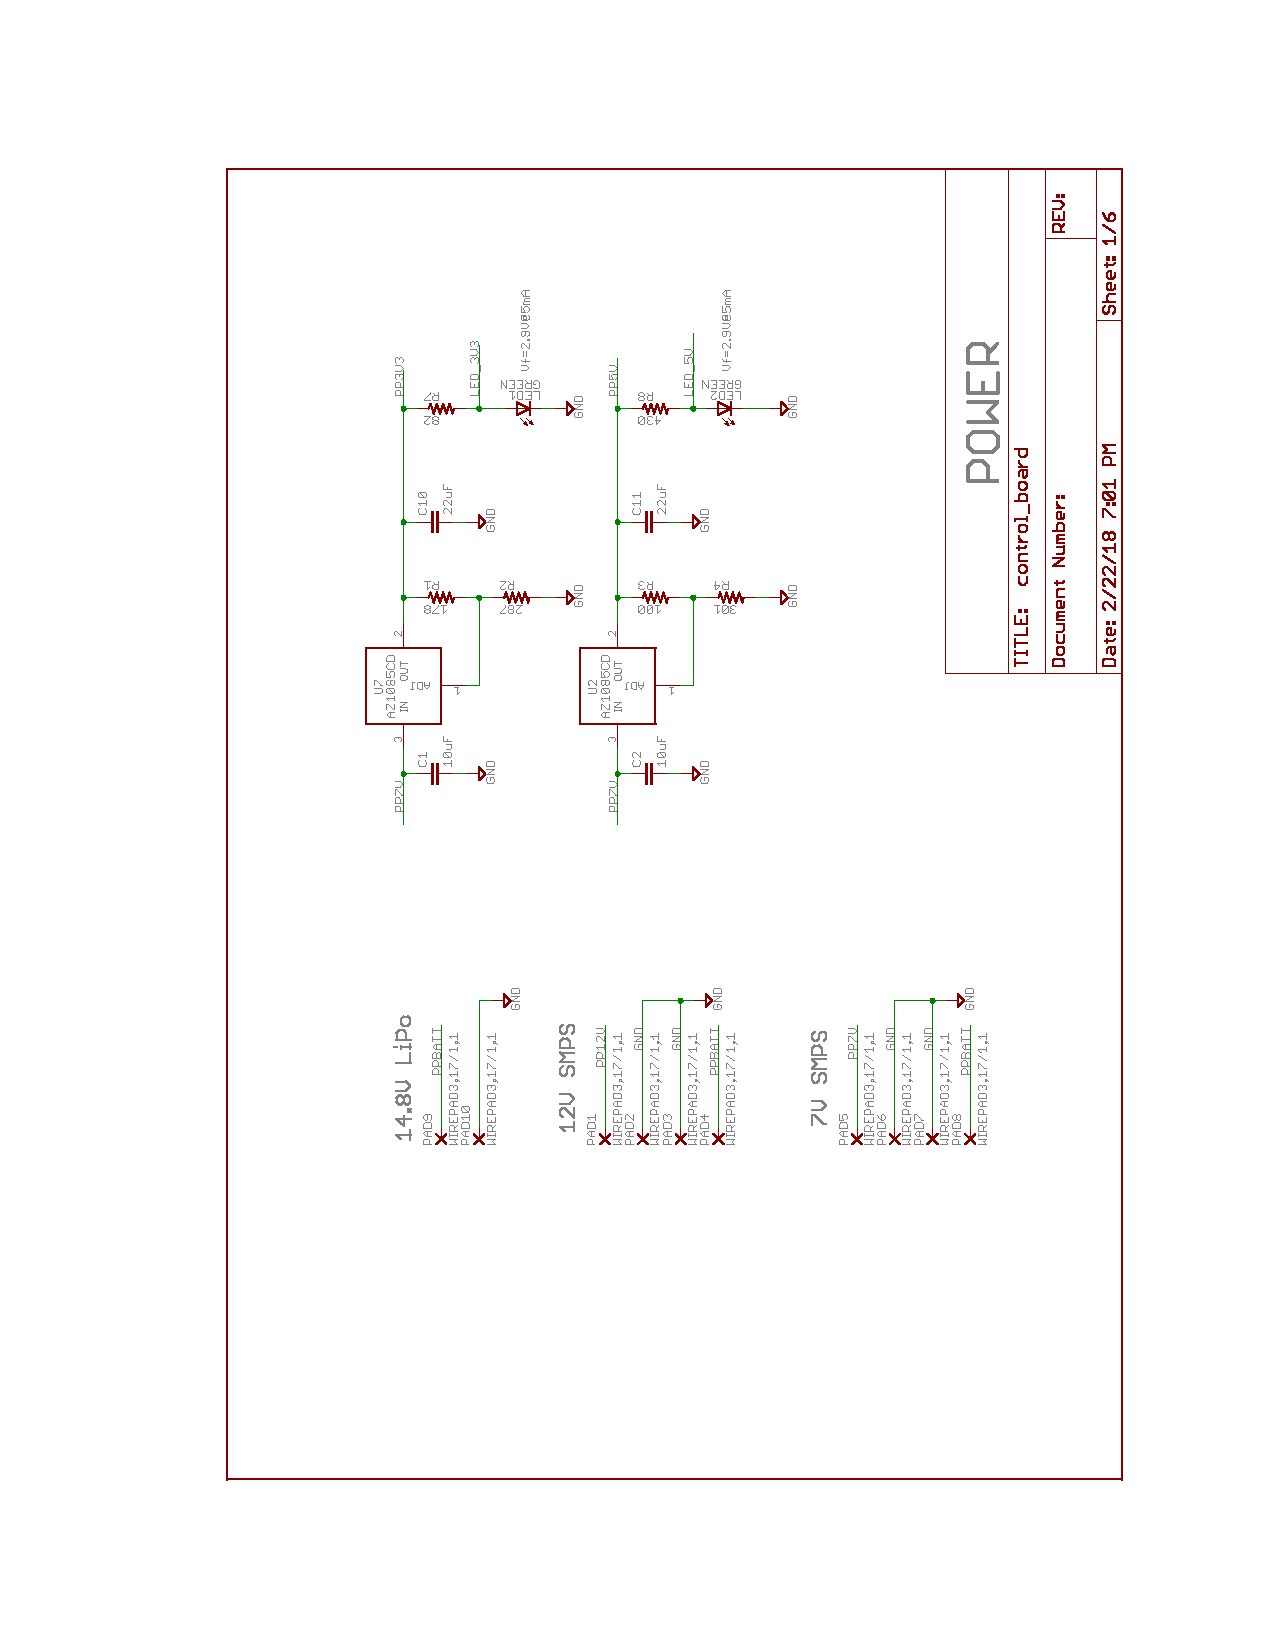
\includepdf[pages=-,pagecommand=\thispagestyle{plain}]{appendices/schematic.pdf}
\chapter{Interconnect PCB Layout}
\label{appendix:layout}
\begin{figure}[H]   % [h] means here
	\centering 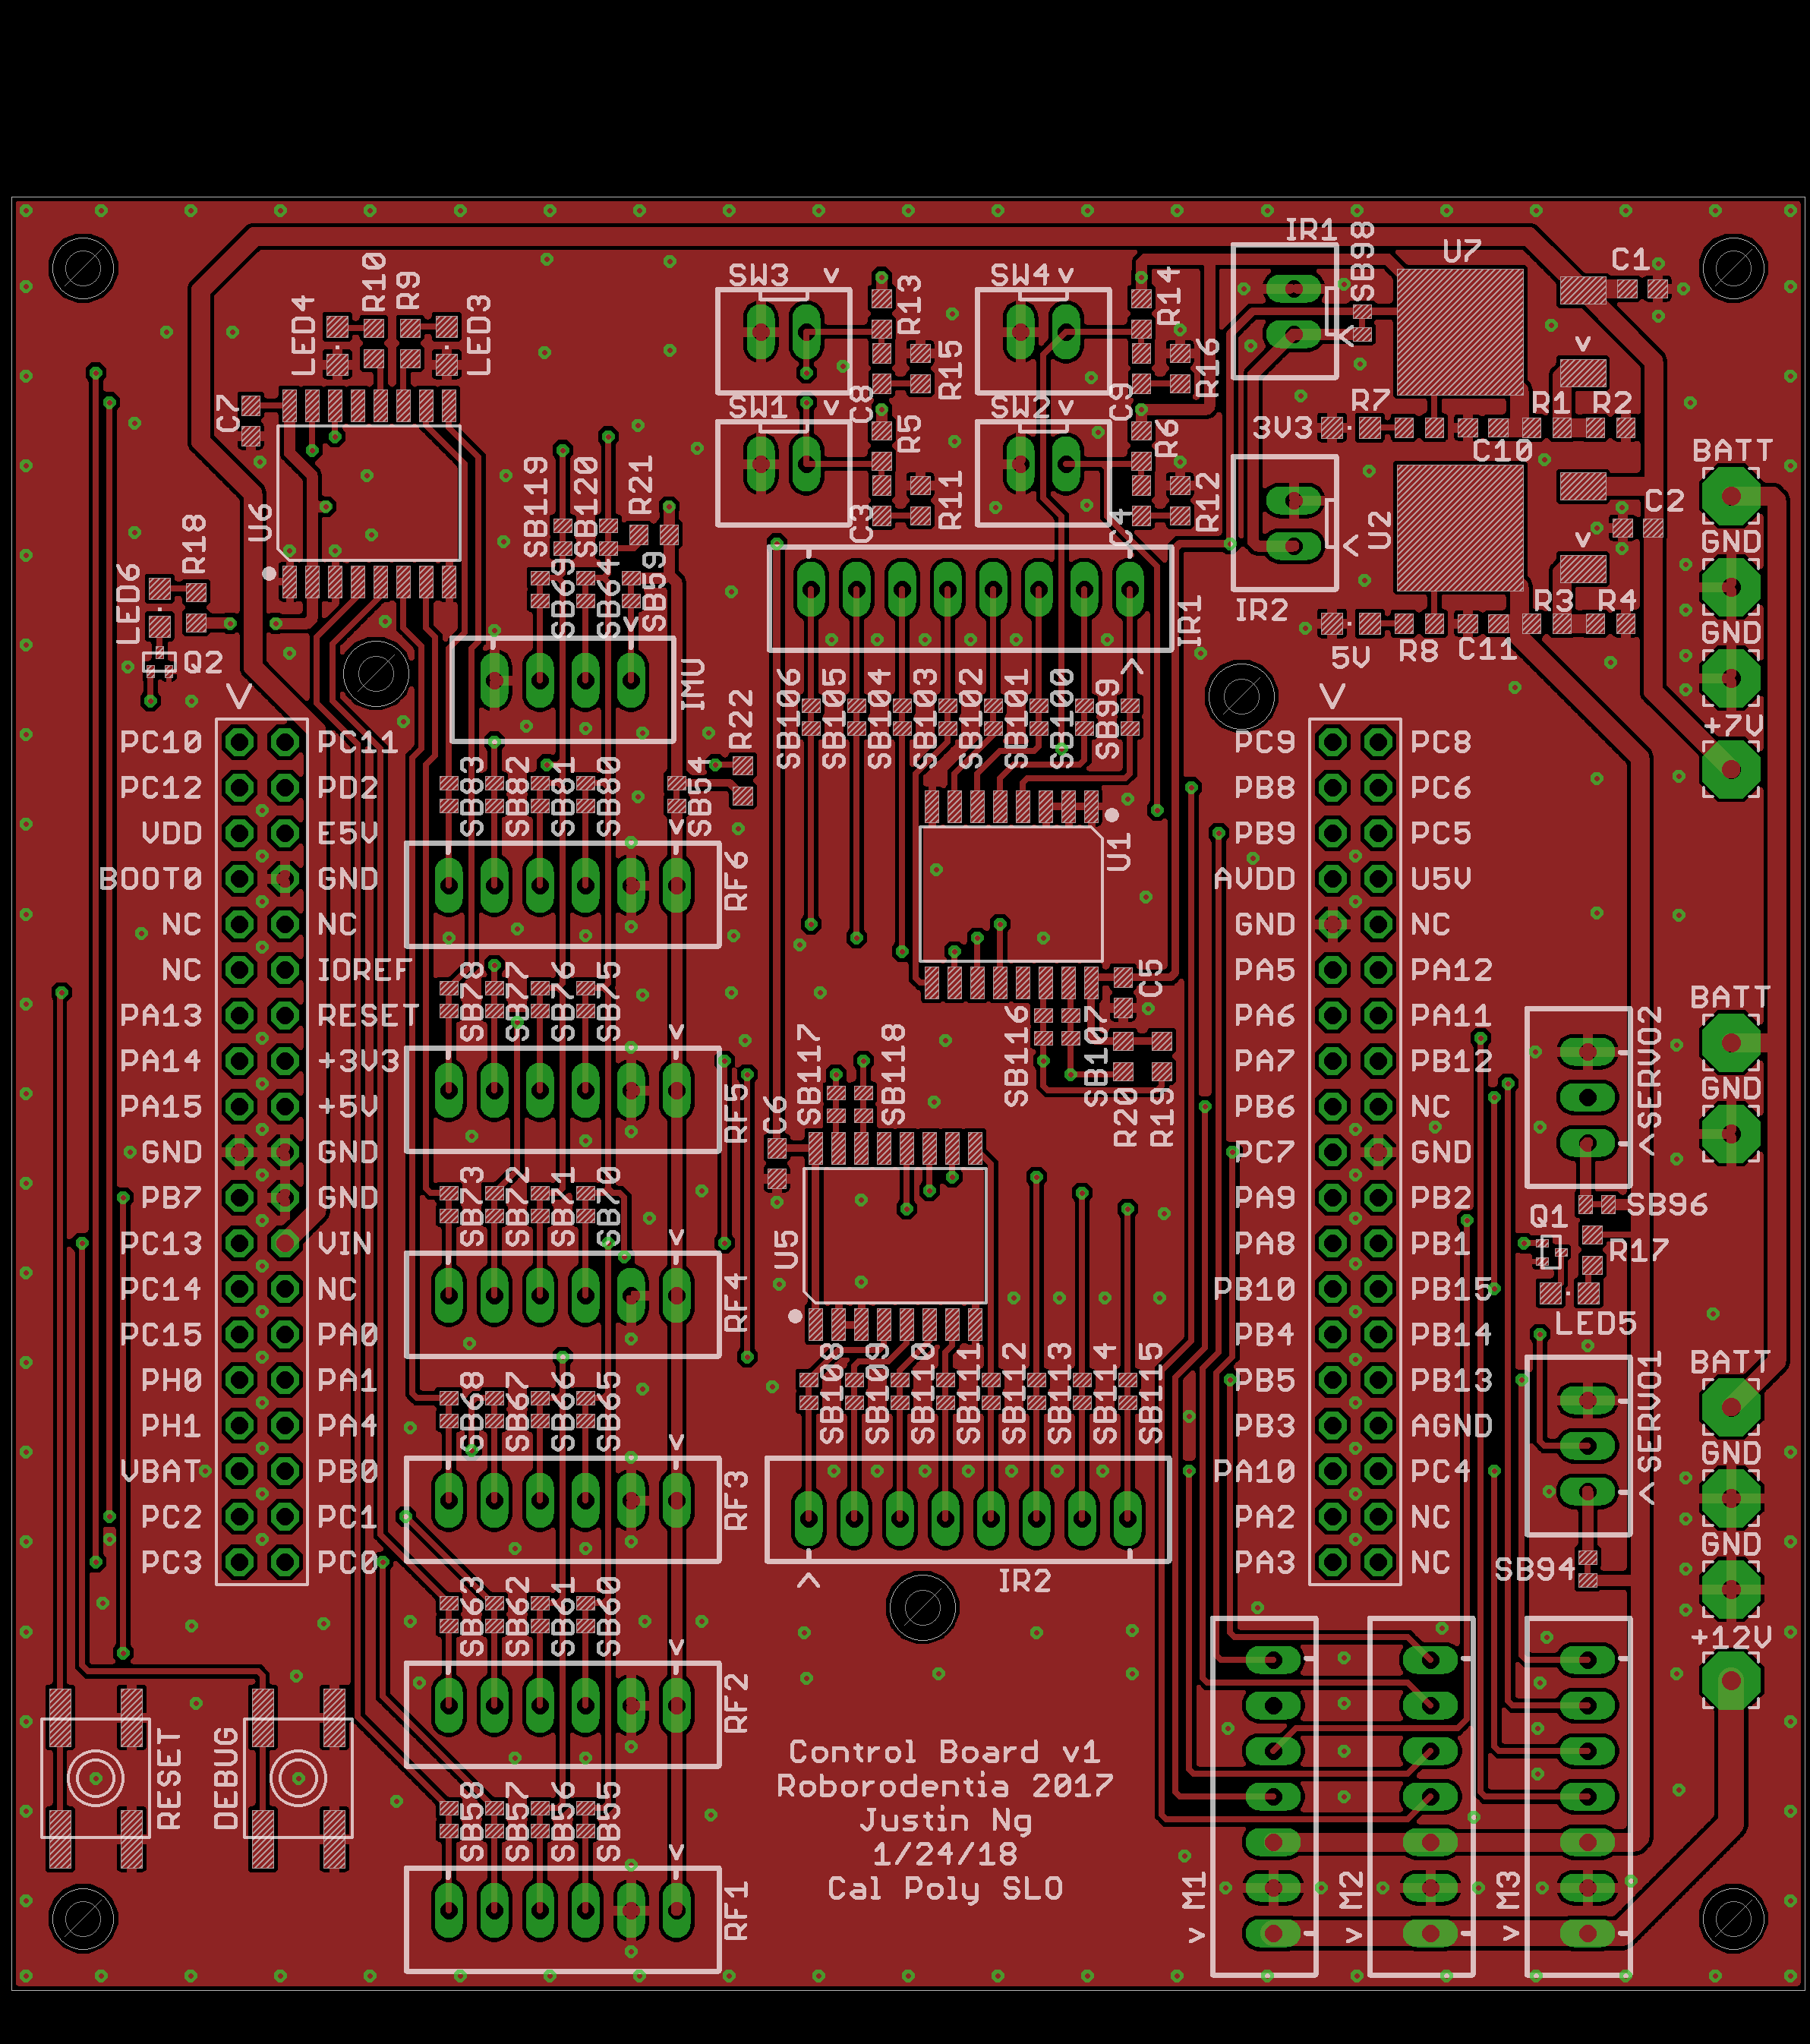
\includegraphics[width=6in, keepaspectratio]{figures/pcb_layout_top.png}
	\caption{Interconnect PCB Layout -- Top Layer}\label{fig:pcb_layout_top}
\end{figure}
\begin{figure}[H]   % [h] means here
	\centering 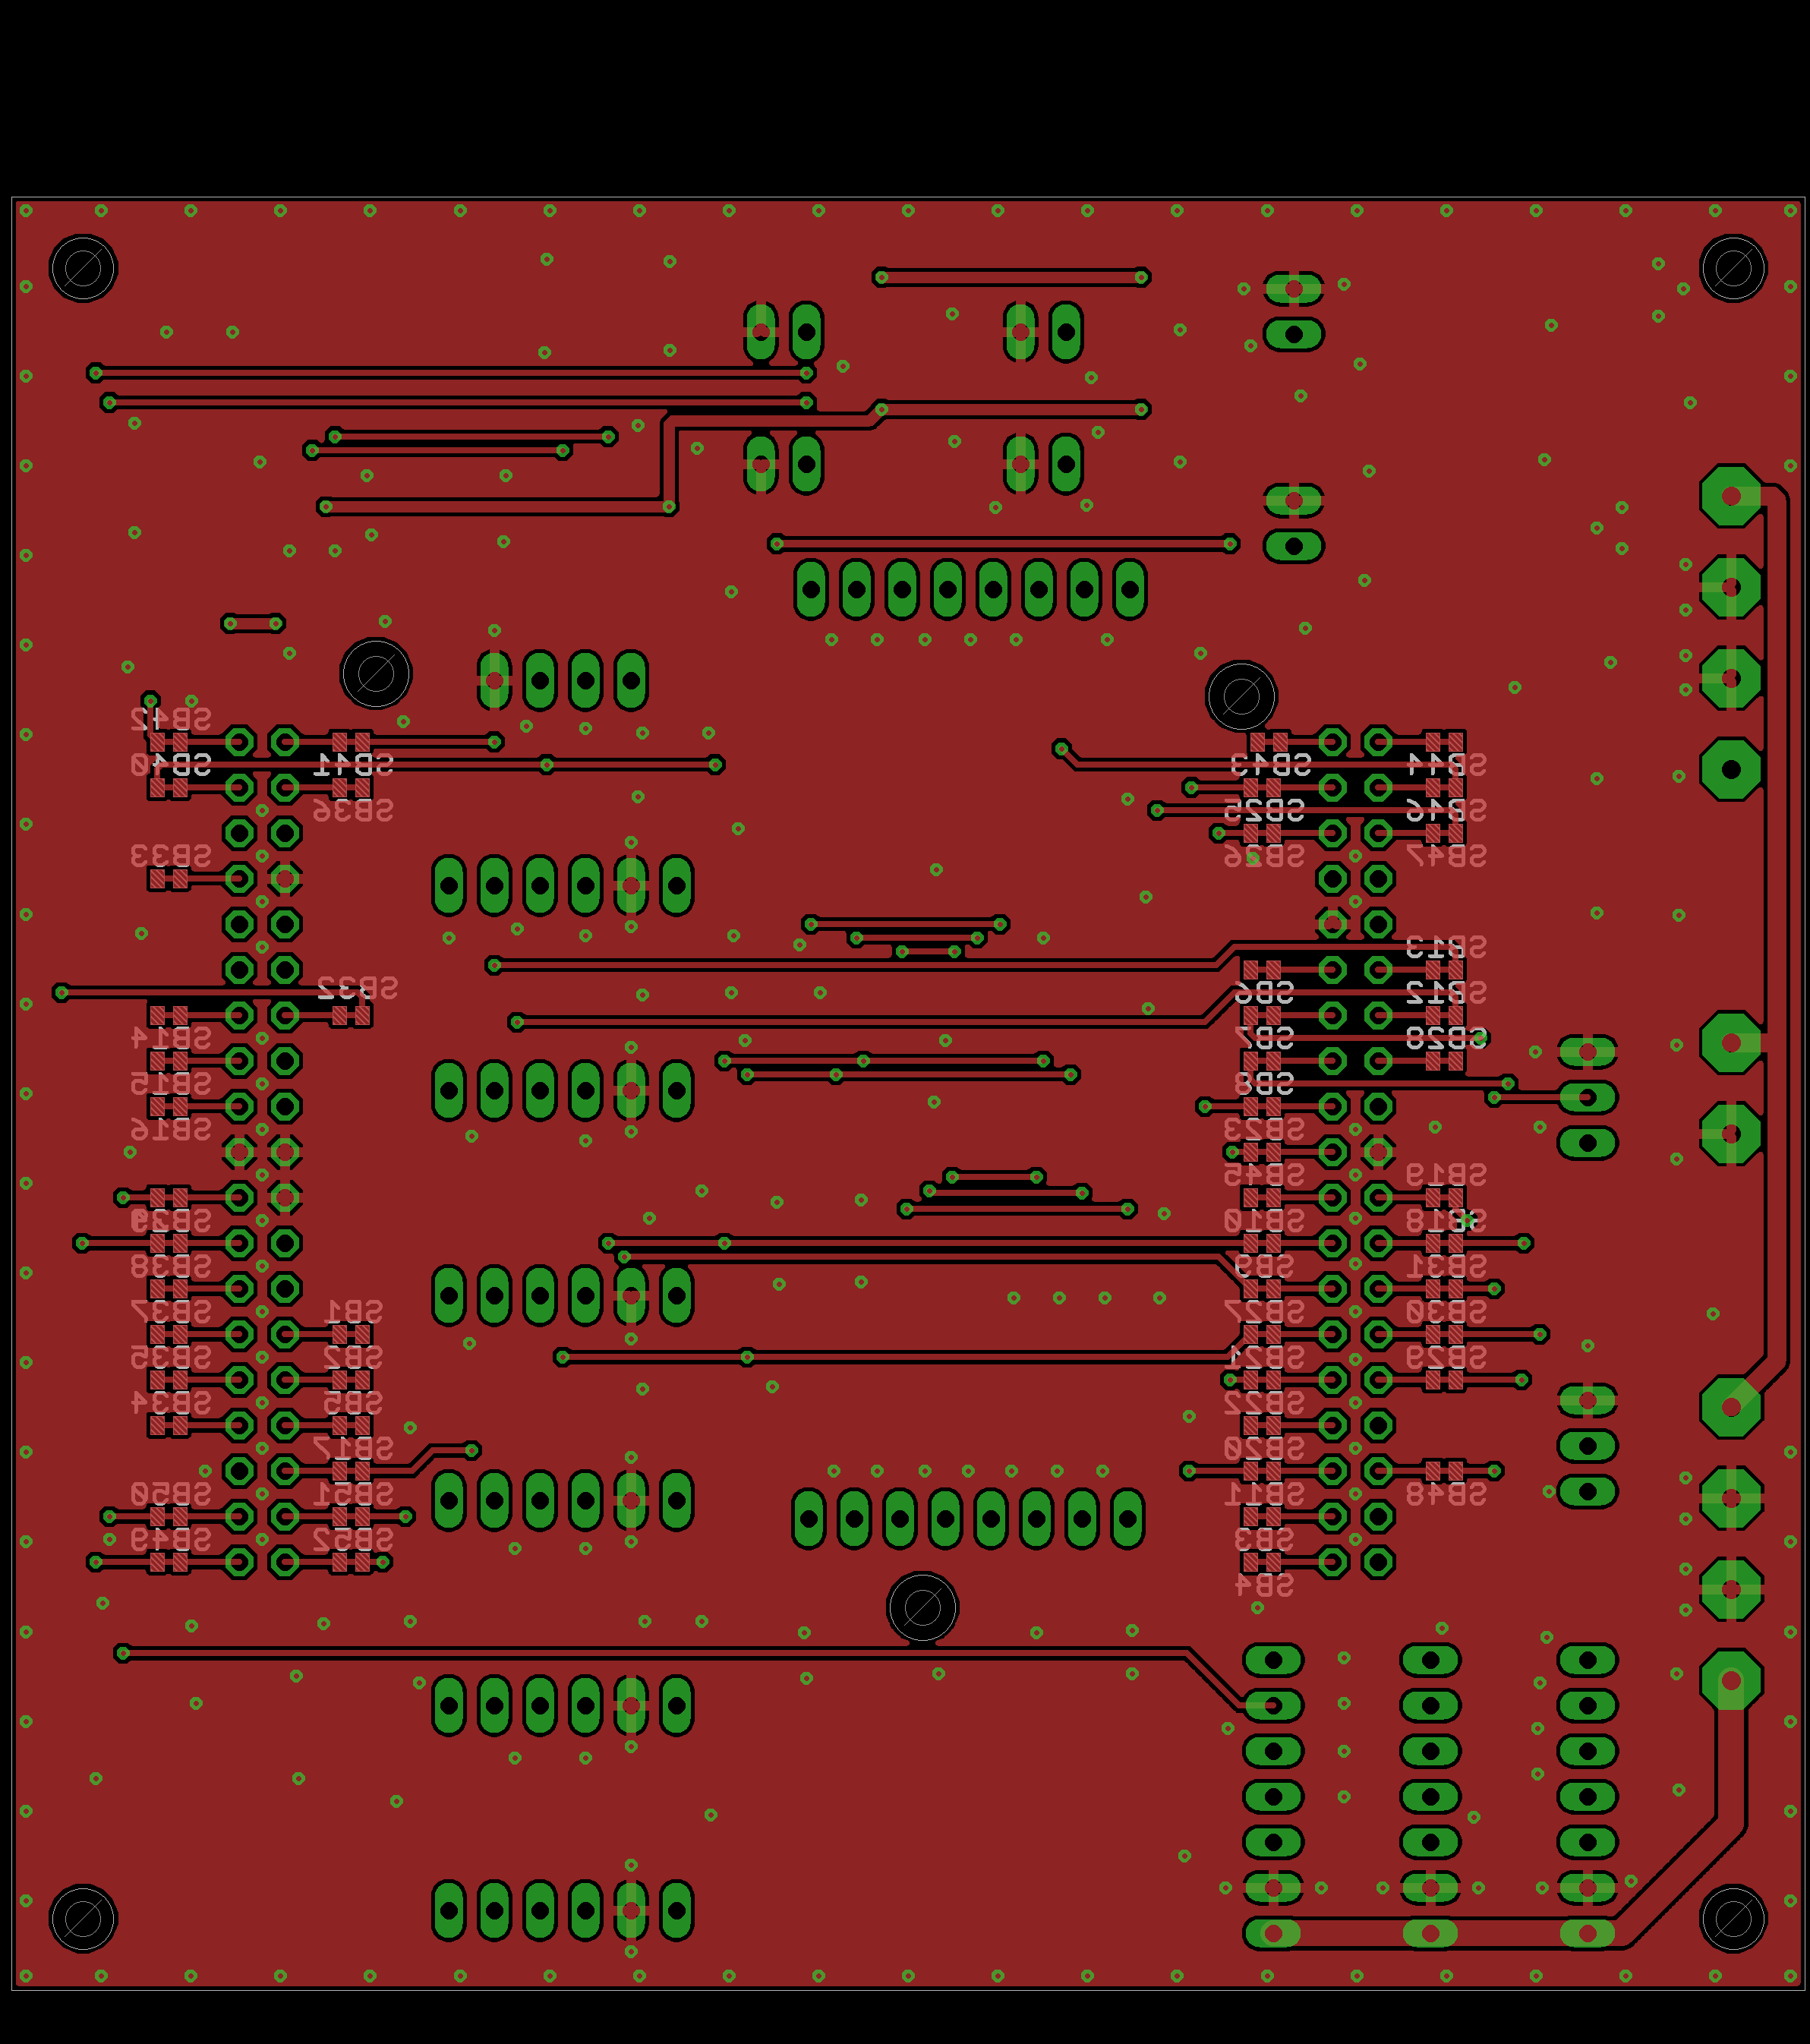
\includegraphics[width=6in, keepaspectratio]{figures/pcb_layout_bot.png}
	\caption{Interconnect PCB Layout -- Bottom Layer}\label{fig:pcb_layout_bot}
\end{figure}
\chapter{Interconnect PCB Bill of Materials}
\label{appendix:pcb_bom}

\begin{landscape}
\small
\begin{longtable}{rrlp{2.7in}p{1.7in}p{1.7in}}
	\caption{Interconnect PCB Bill of Materials}
	\label{tab:pcb_bom}
	\endfirsthead
	\endhead
	\toprule
	\multicolumn{1}{c}{Qty} & \multicolumn{1}{c}{Value} & \multicolumn{1}{c}{Package} & \multicolumn{1}{c}{Parts} & \multicolumn{1}{c}{Description} & \multicolumn{1}{c}{DIGIKEY PN} \\ 
	\midrule
	2 & AZ1085CD & TO252 & U2, U7 & AZ1085C & AZ1085CD-ADJTRG1DICT-ND \\ 
	7 & 0.1uF & C0603 & C3, C4, C5, C6, C7, C8, C9 & CAPACITOR & 445-5667-1-ND \\ 
	2 & 10uF & C0603 & C1, C2 & CAPACITOR & 490-13248-1-NDÊ \\ 
	2 & 22uF & C0603 & C10, C11 & CAPACITOR & 490-10476-1-ND \\ 
	3 & TCA9554A & SOIC16 & U1, U5, U6 & I2C 8-bit GPIO Expander & 296-45456-1-ND \\ 
	6 &  & JST-XH-02 & X1, X12, X16, X18, X19, X20 & JST XH Connector 2 Pin & 455-2247-ND \\ 
	2 &  & JST-XH-03 & X13, X14 & JST XH Connector 3 Pin & 455-2248-ND \\ 
	1 &  & JST-XH-04 & X8 & JST XH Connector 4 Pin & 455-2249-ND \\ 
	6 &  & JST-XH-06 & X2, X3, X4, X5, X6, X7 & JST XH Connector 6 Pin & 455-2271-ND \\ 
	3 &  & JST-XH-07 & X9, X10, X11 & JST XH Connector 7 Pin & 455-2252-ND \\ 
	2 &  & JST-XH-08 & X15, X17 & JST XH Connector 8 Pin & 455-2251-ND \\ 
	6 & GREEN & CHIPLED\_0805 & LED1, LED2, LED3, LED4, LED5, LED6 & LED & 732-4971-1-ND \\ 
	2 & RE1C002UN & SOT416FL & Q1, Q2 & Logic-level N-FET & RE1C002UNTCLCT-ND \\ 
	4 & 82 & R0603 & R7, R9, R10, R18 & RESISTOR & 311-82.0HRCT-ND \\ 
	5 & 100 & R0603 & R3, R11, R12, R15, R16 & RESISTOR & 311-100HRCT-ND \\ 
	1 & 178 & R0603 & R1 & RESISTOR & 311-178HRCT-ND \\ 
	1 & 287 & R0603 & R2 & RESISTOR & 311-287HRCT-ND \\ 
	1 & 301 & R0603 & R4 & RESISTOR & 311-301HRCT-ND \\ 
	2 & 430 & R0603 & R8, R17 & RESISTOR & 311-430HRCT-ND \\ 
	4 & 3.3k & R0603 & R19, R20, R21, R22 & RESISTOR & 311-3.30KHRCT-ND \\ 
	4 & 4.7k & R0603 & R5, R6, R13, R14 & RESISTOR & 311-4.70KHRCT-ND \\ 
	2 & SPST & EVQ-Q2 & SW1, SW2 & SMT 6mm switch & P12955SCT-ND \\ 
	1 & STM32F446 & NUCLEO & U4 & STM32 NUCLEO-64 & 497-15882-ND \\ 
	10 &  & 3,17/1,1 & PAD1, PAD2, PAD3, PAD4, PAD5, PAD6, PAD7, PAD8, PAD9, PAD10 & Wire PAD connect wire on PCB & n/a \\ 
	105 &  & BRIDGE & SB1, SB2, SB3, SB4, SB5, SB6, SB7, SB8, SB9, SB10, SB11, SB12, SB13, SB14, SB15, SB16, SB17, SB18, SB19, SB20, SB21, SB22, SB23, SB24, SB25, SB26, SB27, SB28, SB29, SB30, SB31, SB32, SB33, SB34, SB35, SB36, SB37, SB38, SB39, SB40, SB41, SB42, SB43, SB44, SB45, SB46, SB47, SB48, SB49, SB50, SB51, SB52, SB54, SB55, SB56, SB57, SB58, SB59, SB60, SB61, SB62, SB63, SB64, SB65, SB66, SB67, SB68, SB69, SB70, SB71, SB72, SB73, SB75, SB76, SB77, SB78, SB80, SB81, SB82, SB83, SB94, SB96, SB98, SB99, SB100, SB101, SB102, SB103, SB104, SB105, SB106, SB107, SB108, SB109, SB110, SB111, SB112, SB113, SB114, SB115, SB116, SB117, SB118, SB119, SB120 & Solder bridge with knife-cuttable prebridged connection. & n/a \\ 
	\bottomrule
\end{longtable}
\end{landscape}
\chapter{STM32CubeMX Report}
\label{appendix:stm32cubemx_report}
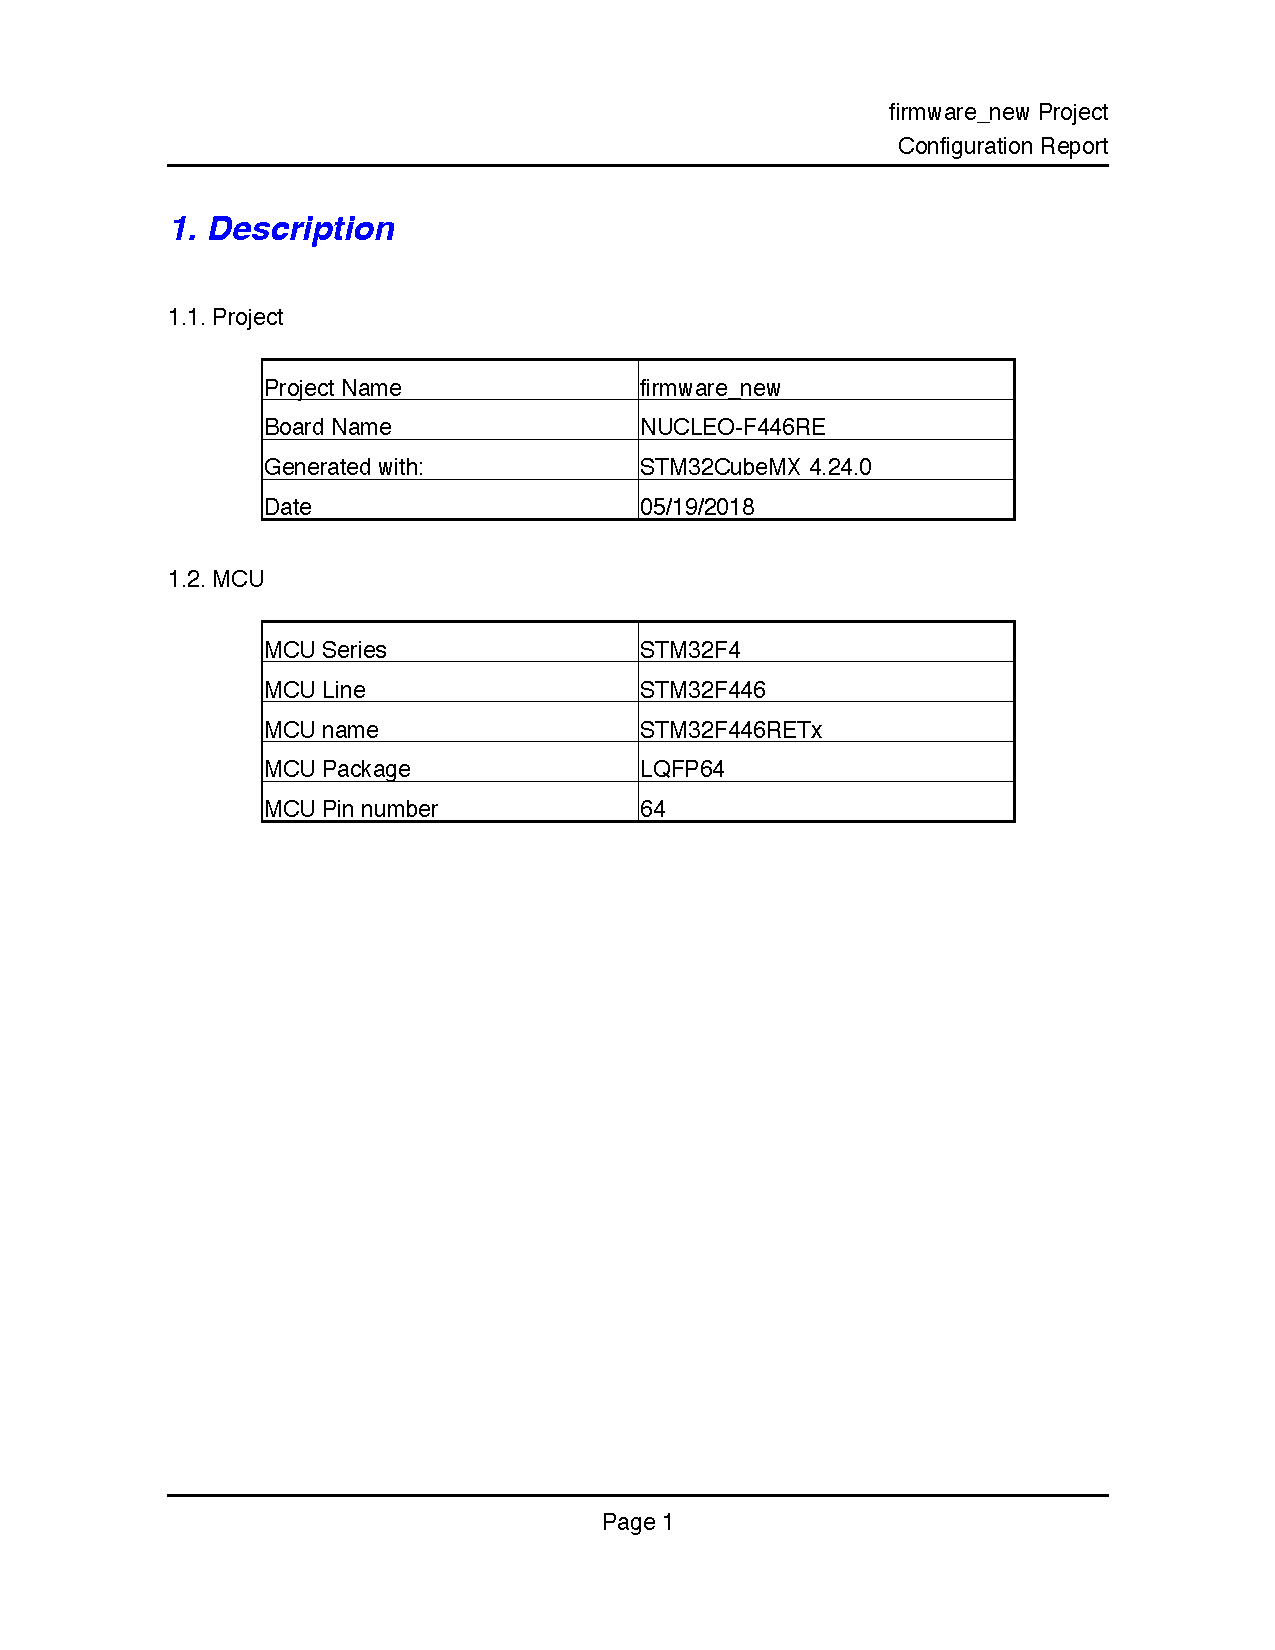
\includepdf[pages=-,pagecommand=\thispagestyle{plain}]{appendices/stm32cubemx_report.pdf}
\end{appendices}

\end{document}
